% universal settings
\documentclass[smalldemyvopaper,11pt,twoside,onecolumn,openright,extrafontsizes]{memoir}
\usepackage[utf8x]{inputenc}
\usepackage[T1]{fontenc}
\usepackage[osf]{Alegreya,AlegreyaSans}
\usepackage{graphicx}

% PACKAGE DEFINITION
% typographical packages
\usepackage{microtype} % for micro-typographical adjustments
\usepackage{setspace} % for line spacing
\usepackage{lettrine} % for drop caps and awesome chapter beginnings
\usepackage{titlesec} % for manipulation of chapter titles
\usepackage{etoolbox}
\AtBeginEnvironment{quote}{\singlespacing\small}
% for placeholder text
\usepackage{lipsum} % to generate Lorem Ipsum

% other
\usepackage{calc}
\usepackage{hologo}
\usepackage[hidelinks]{hyperref}
%\usepackage{showframe}

% PHYSICAL DOCUMENT SETUP
% media settings
\setstocksize{8.5in}{5.675in}
\settrimmedsize{8.5in}{5.5in}{*}
\setbinding{0.175in}
\setlrmarginsandblock{0.611in}{1.222in}{*}
\setulmarginsandblock{0.722in}{1.545in}{*}

% defining the title and the author
%\title{\LaTeX{} ePub Template}
%\title{\textsc{How I Started to Love {\fontfamily{cmr}\selectfont\LaTeX{}}}}
\title{The Anselmo Kiefer Affair}
\author{Eugenio de Arnal}
\newcommand{\ISBN}{0-000-00000-2}
\newcommand{\press}{}

% custom second title page
\makeatletter
\newcommand*\halftitlepage{\begingroup % Misericords, T&H p 153
  \setlength\drop{0.1\textheight}
  \begin{center}
  \vspace*{\drop}
  \rule{\textwidth}{0in}\par
  {\Large\textsc\thetitle\par}
  \rule{\textwidth}{0in}\par
  \vfill
  \end{center}
\endgroup}
\makeatother

% custom title page
\thispagestyle{empty}
\makeatletter
\newlength\drop
\newcommand*\titleM{\begingroup % Misericords, T&H p 153
  \setlength\drop{0.15\textheight}
  \begin{center}
  \vspace*{\drop}
  \rule{\textwidth}{0in}\par
  {\HUGE\textsc\thetitle\par}
  \rule{\textwidth}{0in}\par
  \vspace{.25\textheight}
  {\Large\textit\theauthor\par}
  \vfill
  {\Large\scshape\press}
  \end{center}
\endgroup}
\makeatother

% chapter title manipulation
% padding with zero
\renewcommand*\thechapter{\ifnum\value{chapter}<10 0\fi\arabic{chapter}}
% chapter title display
\titleformat
{\chapter}
[display]
{\normalfont\scshape\huge}
{\HUGE\thechapter\centering}
{0pt}
{\vspace{18pt}\centering}[\vspace{42pt}]

% typographical settings for the body text
\setlength{\parskip}{0em}
\linespread{1.5}

% HEADER AND FOOTER MANIPULATION
  % for normal pages
  \nouppercaseheads
  \headsep = 0.16 in
  \makepagestyle{mystyle} 
  \setlength{\headwidth}{\dimexpr\textwidth+\marginparsep+\marginparwidth\relax}
  \makerunningwidth{mystyle}{\headwidth}
  \makeevenhead{mystyle}{}{\textsf{\scriptsize\scshape\thetitle}}{}
  \makeoddhead{mystyle}{}{\textsf{\scriptsize\scshape\leftmark}}{}
  \makeevenfoot{mystyle}{}{\textsf{\scriptsize\thepage}}{}
  \makeoddfoot{mystyle}{}{\textsf{\scriptsize\thepage}}{}
  \makeatletter
  \makepsmarks{mystyle}{%
  \createmark{chapter}{left}{nonumber}{\@chapapp\ }{.\ }}
  \makeatother
  % for pages where chapters begin
  \makepagestyle{plain}
  \makerunningwidth{plain}{\headwidth}
  \makeevenfoot{plain}{}{}{}
  \makeoddfoot{plain}{}{}{}
  \pagestyle{mystyle}
% END HEADER AND FOOTER MANIPULATION

% table of contents customisation
\renewcommand\contentsname{\normalfont\scshape Contents}
\renewcommand\cftchapterfont{\normalfont}
\renewcommand{\cftchapterpagefont}{\normalfont}
\renewcommand{\printtoctitle}{\centering\Huge}

% layout check and fix
\checkandfixthelayout
\fixpdflayout

% BEGIN THE DOCUMENT
\begin{document}

%%%%%%%%%\begin{figure}[hp]
%%    \vspace*{-1cm}
%    \hspace*{-2.6cm}
%    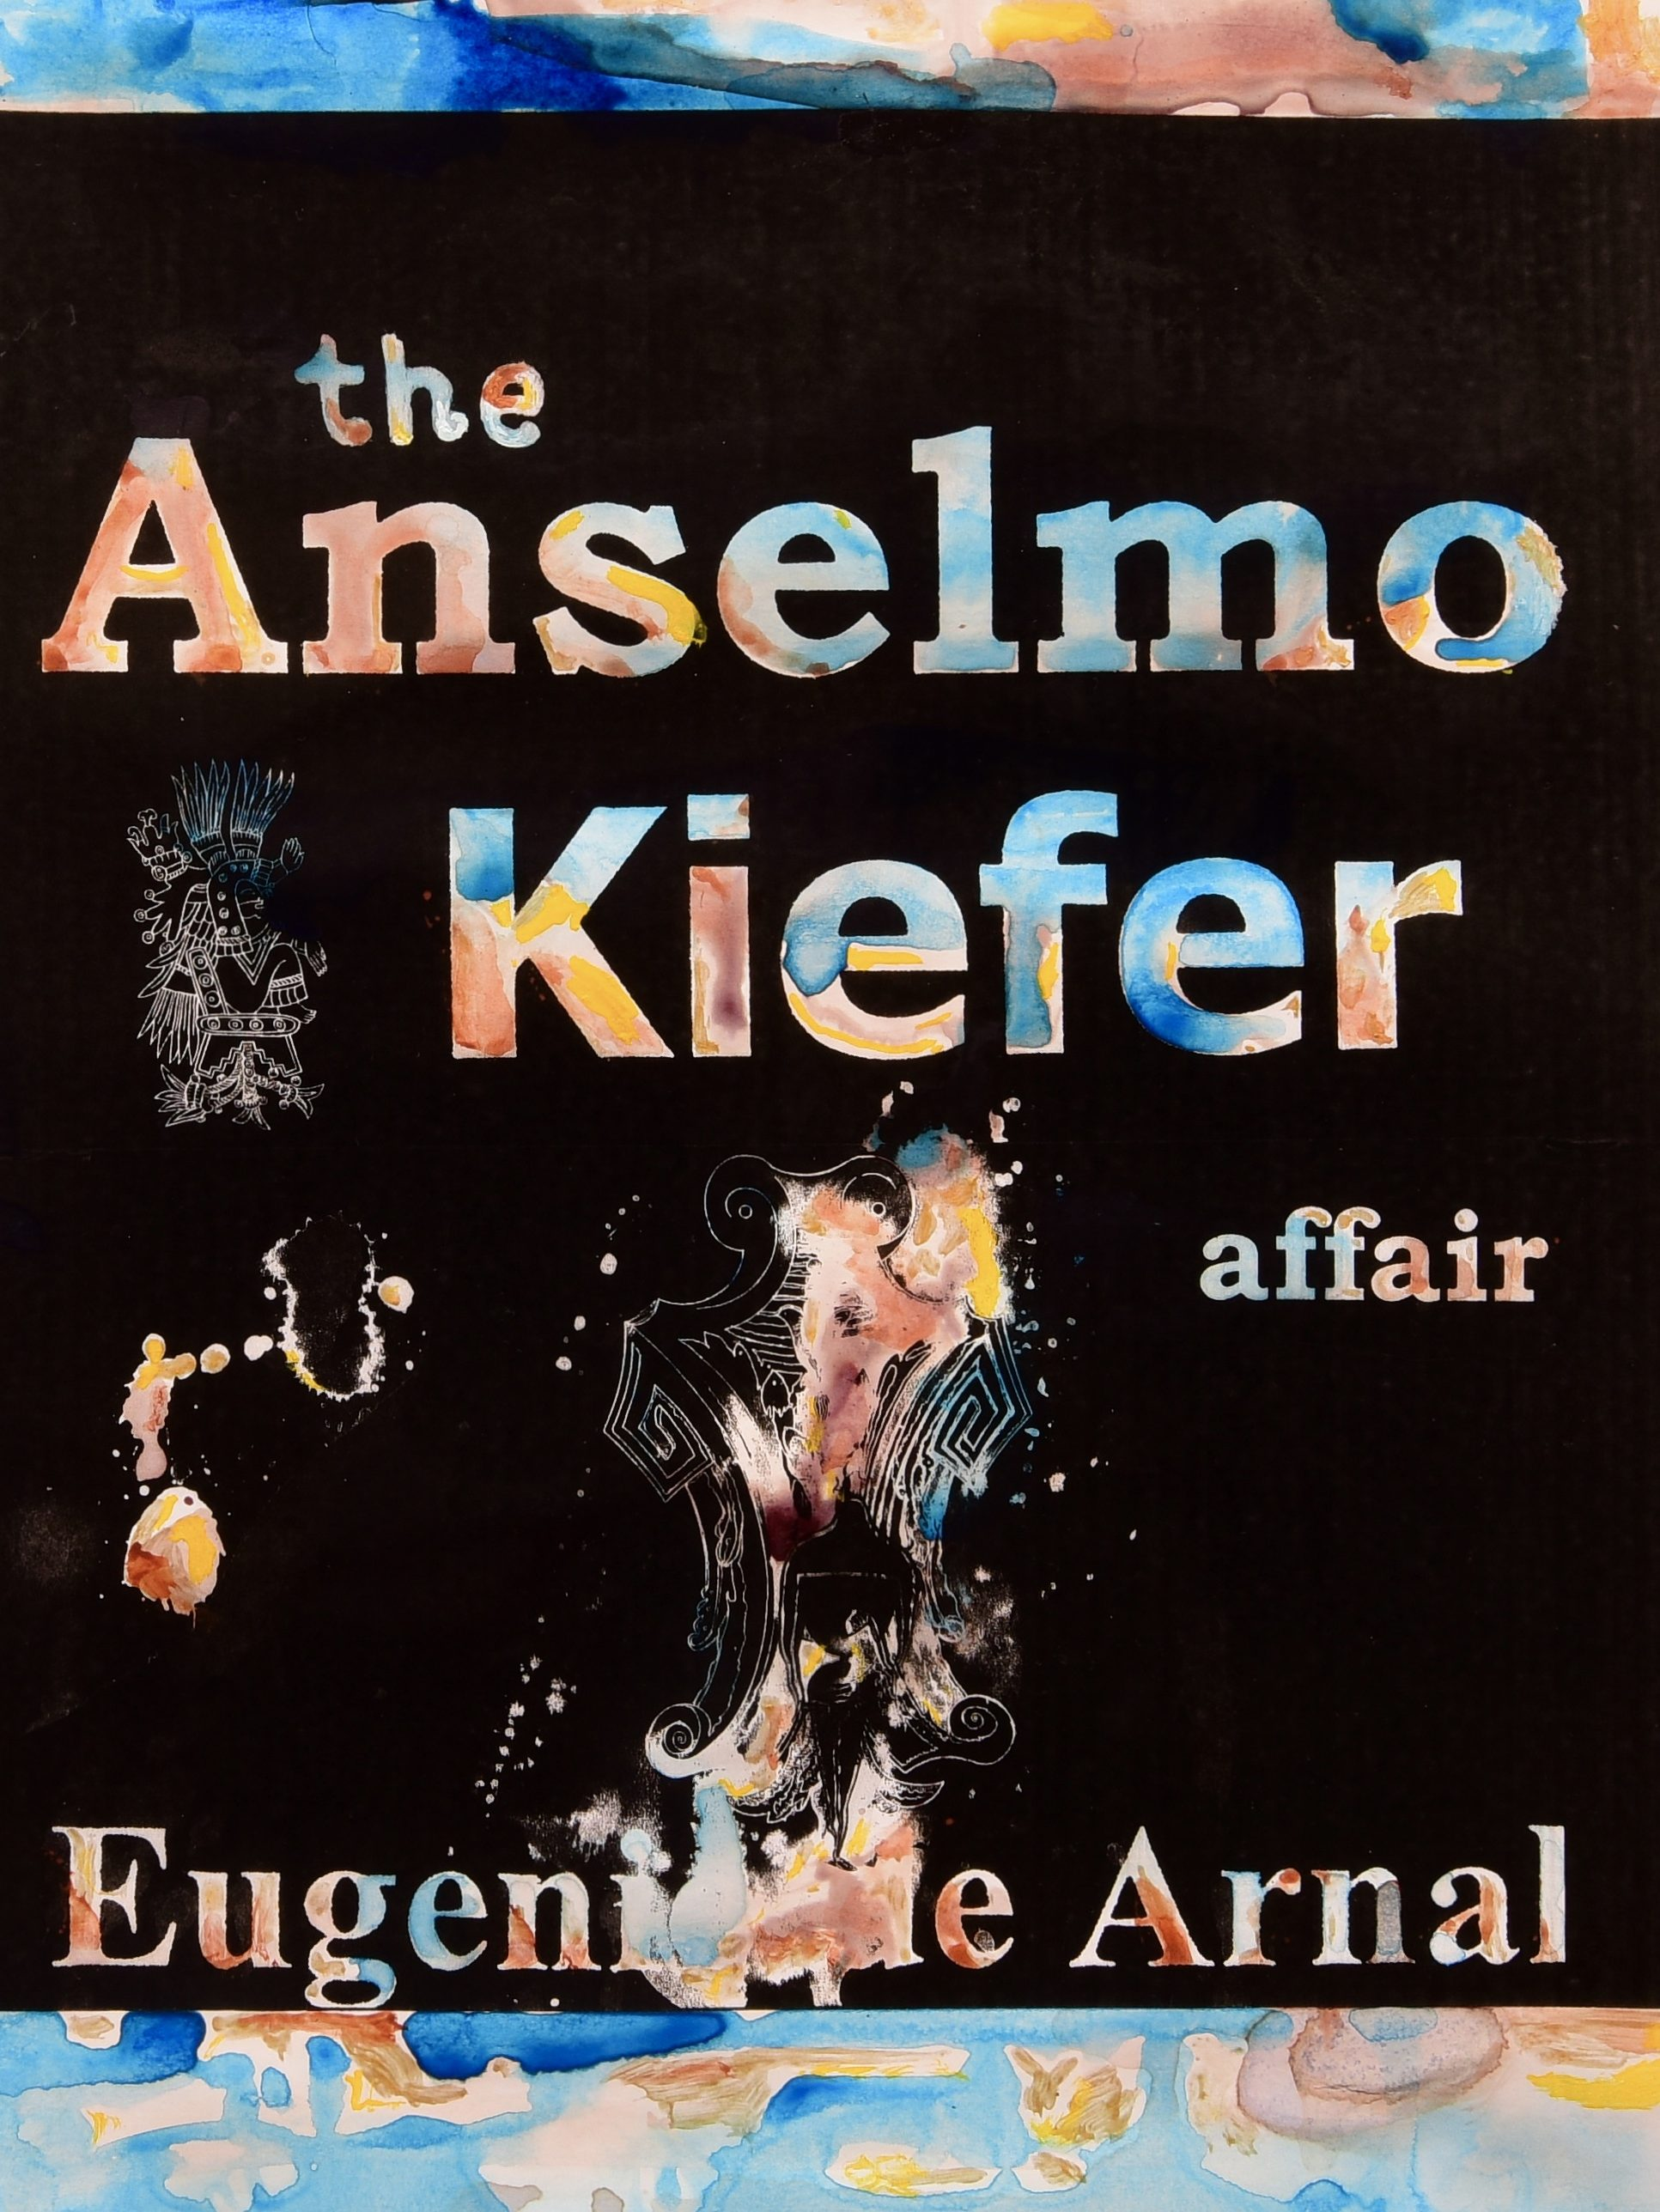
\includegraphics[width=15cm]{./images/cover}
%\end{figure}

%\pagestyle{empty}
% the half title page


%\halftitlepage
%%%%%%%%%%%%\clearpage
% the title page
\titleM
\clearpage
% copyright page
\noindent{\small{This novel is entirely a work of fiction. The names, characters and incidents portrayed in it are the product of the author's imagination. Any resemblance to actual persons, living or dead, or events or localities is entirely coincidental.\par\vfill
\noindent PDF Pre-print Edition\space\today\\
%ISBN\space\ISBN
\copyright\space\theauthor. All rights reserved.
\par\vfill\noindent\theauthor\space asserts the moral right to be identified as the author of this work. All rights reserved in all media. No part of this publication may be reproduced, stored in a retrieval system, or transmitted, in any form, or by any means, electronic, mechanical, photocopying, recording or otherwise, without the prior written permission of the author and/or the publisher.\par}}
\clearpage

% dedication
\vspace*{75px}
\begin{center}
\noindent{Roman à Clef}
\end{center}

% begin front matter
\frontmatter
\pagestyle{mystyle}
% preface
%%%%%%\chapter*{Preface}
%%%%%%\lipsum[100-104]
% acknowledgements
%%%%%%\chapter*{Acknowledgements}
%%%%%%\lipsum[1-9]
% table of contents
%%%%%%\clearpage
%%%%%%\tableofcontents*

\newcommand{\ornamentbreak}{%
    \begin{center}
    -o-%\ornamentleft\quad\ornamentright
    \end{center}%
}

% begin main matter
\mainmatter
%%%%%%\chapter{Chapter One}

\lettrine[lines=3,lraise=0.05, nindent=0.2, findent=0.2]{W}{}hen he saw the photos of the city of Buchen, suddenly many memories came into his mind: Germany. His heart, or part of it, was still there; exactly in Heidelberg. Then by association Egon recalled Anselm Kiefer; the illustrious Master, the formidable Master. The formidable Bull Shit.

How did he meet him? He tried to unite the unconnected threads of his memory. "But how? Well, this is important!" he said to himself.

Wotan, a.k.a. Anselm Kiefer, the genius of grandiloquence of the bombastic pretentious and explosive painting, of eclectic aesthetics, too hybrid, too bastard without draftsmanship. How? Without fear and no pain. Wow! Helter-skelter! Sloppy! All the way! (check it out!) The ghastly, miserably, horrendous portraits of Germany’s Nobles, and the Gettys gave him a medal? (for what?) Who are the Gettys?

His iconography galvanized by horror, and the raw makeshift of his sloppiness, it was a memorable experience where Egon Monte had learned very much from the Barnum of the art of painting in the spotlight of the international world of art! The giant of Walhalla in Buchenwald where more than any Wotan, Kiefer was an exceptional Fafner. A Dragon!

That was a particular, very special, very interesting episode. Everything started like a joke, Egon had read an article in Artforum Magazine, where they were talking about Kiefer and were saying that Kiefer is the artist that is rescuing Germany of the darkness of postwar and he was flaunting them; with cultural values once again, he was making them current, and this was paramount through his plastic pyrotechnics; Germany was reborn from the ashes like a fenix cat. All this was Egon’s liking and he said to himself “I will write to the master”. And he did it, he wrote a complex yet simple letter:

\begin{quote}
    Master Kiefer

    I am a painter, experimental photographer, a saltimbanque, Mexican to the core. I admire Bach, Beethoven, Mozart, Luther, and Dürer, among others. I would like to be in your team. 
    
    References upon request. 

    I salute you my friend.


\includegraphics[width=3cm]{./images/Egon}

    Egon Montezuma    
\end{quote}


He got the address from a German friend and sent the letter like somebody that sends a message in a bottle, from a far and solitary island, his island: Krakatoa to the east of Java, Egon used to call it his 'incommensurable bubble.'

Then after several months, Egon got the answer from the German artist. 

\begin{quote}
    Entschuldigen, die zeit verfliegt 

    Lieber Egon Berg:
    
    Come quickly and we shall talk, it will be an uncommitted interview. I have been very impressed by your eloquent letter. 

    Dein Freund

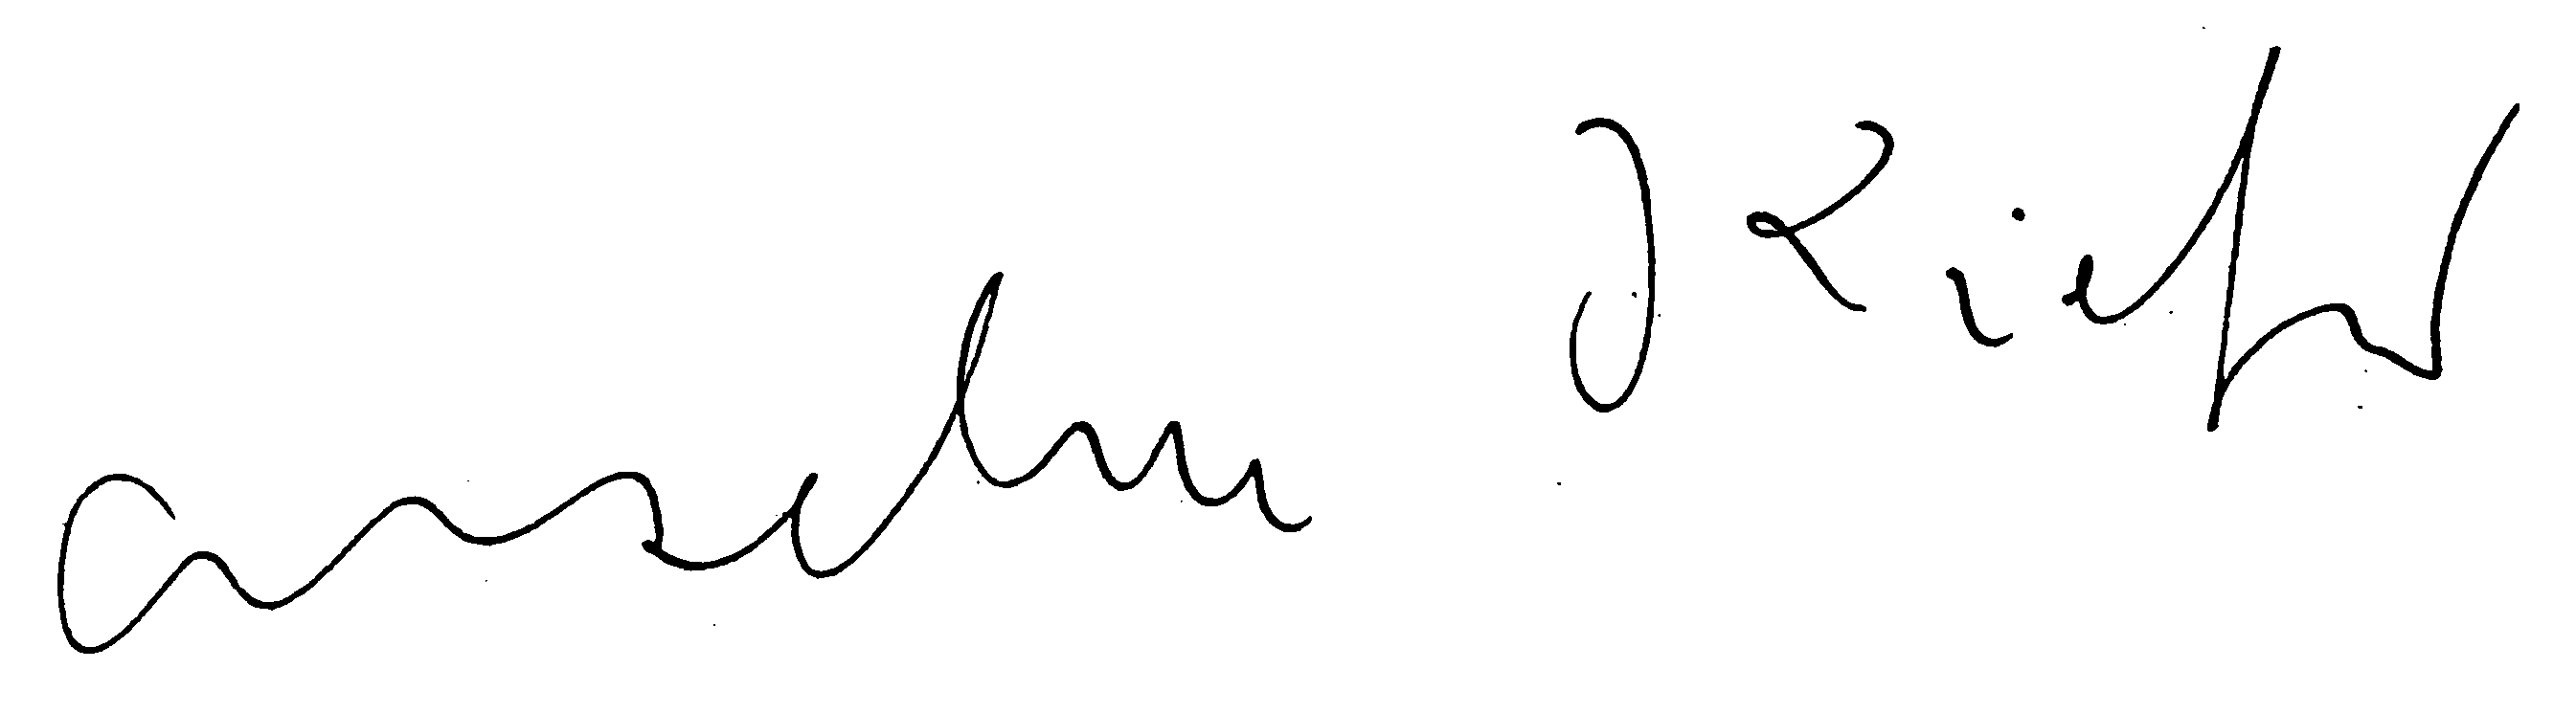
\includegraphics[width=4cm]{./images/anselm}

    Anselm Kiefer
\end{quote}


At this point Egon has a commitment at the city of Heidelberg. He will have an exhibition at Kunsthouse Welker, and he plans meticulously his steps. Make several calls to Europe. This trip will connect him with Kiefer; it will be a great opportunity.

At this time Egon has been working in a series of watercolors and photographs, deriving from the experimentation with chemical substances: Elón, Hyposulfite, Hydroquinone, Ektol, etc and solarization. The result is a group of images of truly mysterious and original effect. The models at times are sculptural figures made with secret manipulations, other times using roots transformed by the effect of erosion found in his explorations, opening his eyes to the mirror of nature. The form, matter, the surface, all is emblematic and metaphor; sex, and its implications; psychological social, politic or philosophical, but avoiding the pornographic trap. Egon is so sure of reconstructing in his Theme the images so worn out and boring of pornography, and his work is a poetical attempt. Besides eroticism is the antithesis of pornography, regardless of sensuality being the Threshold of Death!

At this time occurs the Kiefer exhibition that Lufthansa has brought to Chicago and afterwards will come to Los Angeles, and Egon makes preparations to go and see it. Egon calls Arnold Schifrin, Angelino artist that he met some year ago, and Schifrin accepts to go and pick him up at the airport, offers lodging and very soon they will see the exhibition at LACMA the same day of Egon’s arrival.

Egon confirmed the attitude of the German artist, one sculpture was really a knock-out, it ate his brains, it was the "painter’s palette with big wings", it was great, it was "la chanson du cygne" or the convocation; "elevacione spirituale?" to this traditional painter’s tool, as is the corny bohemian cap and the repulsive attire of the snob. And the obvious, the recurrent themes, references to cultural values and not only German but Mesopotamian, Egypt, the Hebrew tradition, the Bible, Old and New Testament, Osiris, The Kabbalah, The Zohar, The Book of Splendor, etc, a convergence, a river of testimonies that the German Midas was handling some times on target some other times confusedly. All these ideas were making Egon Zuma or Monte, anxious. On top of that, the destruction of his draftsmanship, but maybe because of that, interesting; which make his drawings expressionist and Egon was interested. Then all these aberrations; the imitation of the character of xylography, the touch, the surface imitated with paint, very interesting. There is a correlation of Mexican art and German art, Egon is thinking about Orozco and then, the tonal resemblance of Ricardo Martinez, the rigorous palette towards silky blacks, neutral colors, the sepias and stinky siennas similar in Cuevas.

His symbolism with lead (?) and his alchemy gifts to turn it into gold. Ash; the symbol of resurrection and the straw, lots of straw, right! Straw in industrial quantities. He turned himself into a Wotan-Midas, a comic artist, cosmic and sucker! \textit{Mamón}.

Egon prepares his trip and takes off for Europe in November 1987. He arrives at Frankfurt and already his friend and his friend’s wife waits for him, Elke and Holmer Wolfe.

It is a nice welcoming. Holmer had been in San Francisco some years before, and was Egon’s assistant and apprentice, Holmer was under Egon’s wing and he knew about the experiments with classic photography, then, the manipulation with light and the transition towards the canvas, he was aware of all this. Painting influenced photography, now photography is intoxicating painting. Egon experiments with the manipulation of chemistry, the alteration of certain elements gave Egon the opportunity to create images of exceptional beauty and mystery... then he could transmit them to the canvas; it was a discovery of infinite possibilities.

We think about the realism in photography, and its transition to the abstract, the animation in film, etc, all these elements that are used today to produce painting: the windows to the micro and macro cosmos, positive and negative, the digital age and computers offer the enormous possibilities to create images, images of truly great beauty. These are tools, but the supreme one is the imagination. We go now to the sources, Egon thinks about: Muybridge, Lumiére, outstanding Man-Ray, Bacon, Warhol, or the futurists, Giger, and the kids from PIXAR. 

Egon was interested in all these experiments; his starting point was photography, the manipulation of the silver gelatin structure to get images of sublime beauty and mystery and then transferring them to the canvas.

In Germany somebody was on the same path, but the blindness of this \text it{somebody} and banal interests were creating a void and only Egon knew how to fulfill this void. The aesthetic development of this \text it{somebody} showed certain negligence that only Egon knew. Egon had a strong conviction that he was the one to go further than Richter, although he recognized his attempts and results but without soul or with a dead soul. Richter’s photo-paintings realistic illustrative using a projector of opaque images. Was it progressive or a fact that he didn't know how to draw?

All this discussion and experiments were well understood by both, and for Holmer a grateful experience and opportunity.

After some time, Holmer wanted to go back to Germany and asked Egon for a letter of recommendation. With it, it was possible for Holmer to enroll at the University of Leipzig in Germany. Holmer was at this point satisfied with himself, he had an erratic life in San Francisco and had now found himself.

First thing Egon did when he arrived at the airport at Frankfurt was asking Holmer to be taken to Heidelberg. There he had to deliver the art works for the exhibition at Kunsthouse Welker. After this, and knowing that everything was in order, they had time to change impressions and talk. They got into the Mercedes SL Kompressor 500. Egon mention that his artworks would be framed in a simple way by the gallery. When Egon delivered the \texit{guato} cache to Herr Wiegand, the \text it{galeriste} wrote down a list describing the technic, most of them were photographs and watercolors; some of them had applications of metallic inks and overlays of other elements, others using Man Rays solarization and then submerged into acids. He specified the value in Deutsche Marks.

That same day Egon was free of the compromise with the gallery and now it was the time to call master Anselm Kiefer’s Studio, but before this Holmer and his wife Elke had invited Egon for lunch. Suddenly Egon felt the stabbing of hunger in his stomach and quickly accepted.

The trio Calaveras (?) walked  by Marktstrasse, and Elke suggested to go to a Russian restaurant located in the middle of this tumultuous street with lots of people going through, where the old Germany of cobble medieval stones is mixed with the new cosmopolis of ultramodern business offices. Elke suddenly dragged Holmer... the sun was high at the zenith and now a wave of warm heat was in the air, the day that started cold was now transformed, at last for some instants, into a nice and happy episode.

The name of the restaurant is \text it{Rastputin-Stübe} a very special place and water-hole as well.

"Es ist sehr gemütliches", Elke said. The place was decorated with dark ruby velvet curtains, stained glass windows, and religious icons on the walls... Elka suggested 
\texit{Lamb Borsch} saying that it was the perfect dish to welcome Egon. "Ausgezeichnet", Holmer approved.  

They were hungry and devoured the \textit{Borscht Cossack Style} and drank German beer prepared according by the law of 1516 and only with the finest ingredients and pure water.

Holmer and Egon remembered old times; they drank and talked about the future... Elke follows the conversation and makes the point that her English is not very good; she grew up in East Germany where she met Holmer when he was studying at the University of Leipzig. At a certain moment when they finished eating, Egon, impatient, asks if there is a telephone there? The Alsatian waitress tells them that there is one at the end of the hall near the restroom. Egon got up and followed the indications.

Finally Egon makes a call to the city of Buchen, to the Anselm Kiefer’s Studio. The secretary answered and told Egon that Kiefer wants to see him immediately, if possible the next morning. Egon accepts and from that moment forward, Egon is uneasy and impatient and thinks: what will it be like? This encounter with this sacré-monstre of the international art world?

They got up from the table and Egon asked the waitress for \textit{Die Rechnung}, but Holmer had already taken care of that and Egon graciously said "Danke schön!"  "Bitte schön!" answered Elke.

When they were out, the day is full of activity and is brilliant, they walk in the middle of the people and suddenly they heard “El Condor Pasa”, The well known notes and music of the wind instruments of the high Peru, and Egon stops and remains still for some instants and then… They kept walking. Actually a group of aboriginal people from Peru, dressed with their regional attire are producing this sound, Egon, Holmer and Elke crossed through the group and this people that were starting to gather around there, moved apart... All this occurring right at the intersection of the great Cathedral of Heidelberg on Markstrasse, just near some steps from the art gallery Kunsthouse Welker where the artist will show. Egon passes through the group of musicians and these let him pass, they had stopped playing “El Condor Pasa” and remain stupefied, when they have seen the monarch of The Anahuac’s Empire, or is just a mirage that they had seen the emperor Moctezuma III The Third, for sure! Probably they saw themselves in a mirror that never crossed their minds and never expected all this in the middle of Europe.

The sound reappears as soon as the doors of the Mercedes Benz SL 500 Kompressor were shuttled off, the characteristic sound of the wind instruments of the high Peru, Machu-Pichu the Incaica culture... was in the air.

For now he will spend the night at Holmer’s apartment in Finkelbach, they will go to pick up small Bruno their son, the little boy. Egon was back in Germany, he had been there in two other occasions but now he was there for business and for sure this was exciting, because he mixes business with pleasure. Egon was very excited, the trip had been too much and then the change of time, the jet-lag, had him destroyed, \textit{jodido}. He asked Holmer about what time they will departure to Buchenwald? And Holmer answered that before eight.

Egon said good night and went to the bed that the Wolfen had offered him. It was early and he wanted to sleep to get up fresh to jog. He arrived at 2 in the afternoon at the airport of Frankfort. When they arrived to the house at Finkelbach it was around 7:00 p.m. Egon saw Holmer’s photo-laboratory, it was a small room that had been small-Bruno’s bedroom, and Holmer had fixed it up properly for his needs as a professional photographer.

Then he saw the new collection of photographs that Holmer was preparing, these were “Barns” from the agricultural fields of Germany, very beautiful images indeed! Holmer said that maybe one day he would buy one of those “barns” to convert it as a studio.

Egon saw close range those images, the obturator of the camera had stayed open for long time absorbing the winter landscape the autumn, summer, etc. The different seasons of the year and sometimes the same take. The lenses catches the dynamic metamorphosis that was unfolding in front of the camera. It was poetry, Egon thought Holmer was ahead of the work of M. Wesley, his lens were maintained open for long lapses of time, hours, days and the images were registering, marking the pass of Kronos, and was leaving behind a testimonial phantom.

Then his control in the darkroom, printing on papers like Luminox and AGFA, Holmer was a heavy-weight as a photographer Egon recognized. Caponigro, Adams “The bubble gum kid, Kertez, forget it!” It was so much his praise that Holmer gave Egon one, and he allowed him to choose from that group. Egon choose a beautiful one, the one that he kept for a long time very well framed hanging on the wall in his castle of ID, and for sure at these moments he doesn’t know where it ended-up. Perhaps Basilio knows, but where he will be this “boshito” from Yucatan?

Finally he said good night and went to his room it was, Elke’s dormitory and Holmer; the host insisted that they will sleep in the makeshift ship Bruno’s dormitory. Fortunately there was an exit from the bedroom and a stairway that went down to the small patio and from it,  a door to the street.

Egon was very excited and wanted to write until 11:00 that night. Now he was tired and prepared himself to go to bed, he turned the alarm switch and turned off the light.

The alarm rang at 4:30 German time and Egon opened his eyes and jumped out of bed like a spring, he turned on the table lamp and got dressed for running. He didn’t sleep very well, he was still excited for all the developments. It was very cold but the cold was nothing. The cold peeled his teeth! \textit{Le peló los dientes}.

He peeked from the window to the outside and saw the near street that was brilliantly lit. When he was ready, he dared to go out and felt the tam tam of his heart. When he was on the ground and stretched and regained his breath, he flexed his legs, turned his body in tension. He said to himself that he will run for an hour, he wore his gloves and squeezed the hard rubber ball, he pressed hard

He started to trot and followed the line of lights that seemed to have no end. He realized the frozen-zephyr sky and kept running trying to maintain a perfect balance. He tried to memorize houses, buildings, parked cars he saw; the Audis, Mercedes Benz, Porches, etc. The cold air refreshed his head. Suddenly it started snowing as in a Walt Disney’s poetic-film. He looked upwards and saw how the snow plumes were falling and his butt shrunk, \textit{se le arrugó el chico terrible del barrio}. It was a young snow, crepuscular, inoffensive. He kept running and saw the vapor of his breathing, he checked the phosphorescent lights from his wrist, on one of his beautiful hands. At that moment he turned trying not to loose his track and kept going. 

He remembered Kiefer’s face the only ones he knew by the press and movie magazines; in some he looked like a handsome Lotario, daring and intrepid, premature alopecia; in others an insurance salesman or a geography teacher from a rural primary school, others as a shark lawyer, voracious irremovable. The clock in his mind ordered him to check his “Chaos watch”. It was around six and he decided he should go back, he turned at a corner, the dark landscape always changing like a Kaleidoscope. He repeated to himself that he should return and turned to the right, suddenly he didn’t recognize what he obsessively tried to etch in his \textit{mollera}. He turned again at a corner that he thought he recognized so sure that it was the one, but now he was in front of a great mansion in the style of the arquitecture of Andreas Schlüter. The alarm started to sound ferociously, like in hell! Egon felt lost but kept running, scared because the fucking alarm kept sounding madly like if he was in the middle of Germany at war. Egon thought to see ridiculous ghosts, \textit{chocarreros}, and kept running, scared. He could not find Ariadne’s thread, and he felt himself a Minotaur lost in the labyrinth of solitude. He landed on the esplanade, and his desperation worsened. Fuck!! How Horrible!!  Everything was unknown. The sound of the alarms went vanishing little by little in this cruel and cold morning. He was like a shark in the snow, he knew he should keep moving, otherwise \textit{se lo carga la tia de las muchachas, la chingada, claro}! The cold intensified: the fucking hyperthermia was around the corner... for sure!

He had to return and shower and be prepared to go down to have breakfast and get ready for the trip with Holmer to Buchenbald. He kept moving like a boxer, stopping to decipher street names. He tried to remember... what angst..! The name was Rothenbergastrasse 6121 and he couldn’t find it. His watch was eating the time like a caterpillar eating the leaf of a tree, and he stopped. It was getting late so he decided to run in the opposite direction. He felt himself ridiculous and stupid. How was this happening to him in a small city, a city he didn’t know?

At last, he recognized a car that was parked in a strange way. It was a Porsche Targa 911, like the one he had many years ago in San Francisco. By association, he remembered Dena "Pushky" Roberts but those memories belong to another reel. He jumped!! That was the street, he was happy as a clam. Now the street was covered with a white cape of dangerous snow, like a checkered chess table with white pawns, so he ran cautiously.

\ornamentbreak              -0-

When Egon came down for breakfast, Holmer was already reading the newspaper, and Elke was preparing the food. Egon was very impressed when he saw the table, everything was ready. It was a very German breakfast: butter, cheeses, honey, molasses, sugar, fruit, tea. The salmon in fine slices, several kinds of bread, black integral, pumpernickel, terrine de porc. A coffee pot of hot and steamy rich coffee, the marmalade of blackberries, orange juice etc. Everything jammy, aromatic and luscious.

Elke was so nice and discreet, the little Bruno resembling her, a good kid; well behaved with good manners, no tantrums, eating his cereal, getting ready for Elke will soon take him to the Rudolf Stainer school. Egon observed this tableau and was jealous for one minute; he had always wanted to have a son and name him Mistral Huitzilopochtli, and he sighed.

They had breakfast and discussed politics. Europe also saw Reagan as an asshole with his ridiculous tinted hair and his cartoonish behavior and neoconservative ideas taking his country to bankruptcy where then the "Buches" will follow suit, Draconian Retrogrades as well!!Criminals Draconians!!

The time had come to say goodbye to Elke and the kid. Holmer had the Mercedes ready; he filled the tank with petrol Diesel.

Holmer showed to be a good driver, speeding 200 km per hour or more on the Autobahn in that beautiful muscular Mercedes SL 500 Kompressor and Egon there, tied up practically to the leather seat and listening to Kraftwerk or Ute Lemper singing the Falling Leaves or the Blue Angel in French. Egon loved it! By that time, the snow from the freeways had already been removed and the traffic was getting congested, other autos running faster or at the same pace while others were falling behind. The German landscape so special, well taken care of; the hills, the winter trees like skeletons, grayish, and the aluminium of the sky resplendent. Egon saw signs and strange lettering, he had studied the german language, but sometimes, the most, for him all this was incomprehensible… the auto rolled fast and silent, only the music was a present, and Egon saw Holmer so formal and demure, he was not anymore the erratic kid, so noisy and undecided, the one that used to smoke pot at any time indiscriminately in Caroline’s house while the TV was making a lot of noise; the volume all the way up covering or treating to cover the screams and squeals of her son; the terrible Terry; when he turned for no reason in a kind of an uncontrolled maniac. All this was happening while Holmer fuck Caroline and at the end the kid, Holmer and she were passed out by the effects of the Cannabis, the TV at this time will be only turned off when Holmer or Caroline got up eventually to go to the (Orinoco) restroom to hang a lizard (pee)… Holmer used to tell his problems and the maestro was only murmuring “m...m...m...”

The distances in Germany are relatively short if we compare, one can move in a short time from one point to the next point of the country, and obviously in a craft like Holmer’s, supple, comfortable and fast. The Mercedes was flying, then he turned, switch to another runway of the autobahn and there they were going, it seems that Holmer knew very well all the freeways and directions. Egon could see Holmer’s yellow gloves maneuvering the gears with precision and experience, now Holmer behind his smoked spectacles, so serious and efficient.

The tape was repeating and Egon asked Holmer if he liked classical music? “Ja, Natürlich!”  H. answered and he showed Egon the compartment full of music tapes. Egon chose “Die Zauberflöte”, Holmer showed how to put it in the deck Blaupunkt. The space of the cabin was full filled with the mozartian sound and they felt the energy when it came to a climax….. in the aria “The Queen of the Night” sung by Cecilia Bartoli, Egon felt the rupture and recalled the Contessa Erika Farnsmayer, when he closed his eyes.

When “The Queen of the Night” ended, suddenly they saw “Buchenwald Gerade Aus 20 Km” and Holmer slowed down the speed, The Mercedes took the ramp to the right, then it followed by a road that was flanked with very high cypresses. The splendorous morning, it was about 9:30 when they arrived at Buchenwald, Holmer consulted his bag of maps and took the one that was telling them where exactly they were, then he turned left and went for some minutes and said “we are close, it could be little bit ahead…”  He tried to find the card that Egon gave him and then read:

Dieselstrasse 2 Buchenwald… They saw a police patrol that was parked by the side of the road and drove close and asked to the “Polizistin” the right directions. These guys very kindly guided them to the door of the castle of Wotan’s madness, it was just there, around the corner.

Holmer got out of the car and went to press the ring and they waited… Egon started reading the exterior of the building very carefully… Suddenly the gate started to slide, running over the bearings, almost in silence mechanical… It was about 10 in the morning, when the gate was open, Holmer want back in to the Mercedes and then rolled in like in cushions. Egon saw in focus special details; over the ground there were something like cobble stones and over them big lead plates, the wheels rolled over these plates and the tracks were printed on the plates with no doubt. Egon knew it, because he felt how the lead gave up... to the cars weight without noise, then Egon follow the dots and murmured “lead, m, m, m..?” 

When he stepped out of the car, by then in front of the main entrance he confirmed that the lead reached up to the door of the building and the edges of this lead looked like they were sculpted, resembling sea waves, “what was the purpose? maybe the Red Sea? But this is a contradiction!” 

Egon remembered all these details, lead, the modern building with no character, only a box, simple, a geometrical form, very ordinary, its aspect only functional, industrial, big, Egon wanted to read the characteristics that would show the exaggerated geniality that was publicized  by the yankee press, and he couldn’t see anything extraordinary.

The executive plenipotentiary secretary gave them a warm welcome, she said they were waiting for him already and added that her name was Wanda Bolanski and she continued saying that Master Kiefer will arrive in few minutes, she asked them to sit and offered them tea.

Egon and Holmer and Miss Wanga? Sorry, Wanda brought the service on a silver tray Egon recognized the service; it was ceramic by Rosenthal, so exquisite, and the tea turned out to be marvelous; some sort of Chinese tea that grows far away from the desert Gobi and is gathered and harvested by small spider monkeys, and it is brought to the towns. Well this is what Wanda told them, Holmer opened big his eyes and his drool fell to the floor (?).

The fucking cold stayed outside, the warm liquid of this tea was caressing the beautiful Egon’s hands and at the same time was going down his esophagus, to his tummy now smiling. Holmer sat seriously and started leafing through the “Stern” magazine, and then he did make a sign to Egon, Holmer opened the magazine exactly where they were publishing photographs of Anselm Kiefer and a big article where he was championed in an exaggerated way. Egon made a gesture nodding, while he was inspecting everything with his X ray vision, corners and details from this office that looked more of, like an architect’s office than an office belonging to a painter and sculptor, very utilitarian and simplistic.

It was strange! Only big blue-prints on the walls. Egon came close and read: Amsterdam Museum lower plant, all in classical indigo blue, the drafting in negative, parallel coordinates and transversals, and the esoteric language, length, altitude etc., everything in meters and not only one plan of one museum but several; Museum of Modern Art of New York, of the Museum of Paris, Sydney, Tokyo, Australia and a bigger one of the Tel-Aviv Museum of Art. The office furniture ultra modern Bauhaus gray and black leather, the white desk, shelves, archives, telephone, etc., everything impeccable. But no paintings, no sculptures, no photographs of art pieces, how strange?

Then Wanda came close and talk to them, she said that her roots were czech. Egon tried to recognize her with the photograph of the “Shulamita” that he saw at the exhibition in Los Angeles, the features were the same but in the photograph she looked innocent like a fly trying to play death, hypocrite and inoffensive. She couldn’t smash a plate, perhaps all the china (?).

Suddenly the white door opened and appeared one of the assistants of master Kiefer, he presented himself, his name was Georg Mandelbrot and welcomed them. Egon make a guess; probably 25 years old, well dressed, very german very European; heavy cashmere overcoat, burgundy pullover, black Levis and sturmtrupper boots. When he went away he made the sound with the heels and Egon and Holmer were impressed, he disappeared but before that he gave them a warm welcome and said that it was a pleasure to know them. 

Not until one hour later master Kiefer appeared, he introduced himself and cordially he showed the enormous first gallery of the studio. It was a tremendous shock, what happened? He tried to impress them? When they passed through the threshold of the simple, ridiculous impersonal and cold office to the great gallery, they saw, when the door was open, Egon could see the enormous space and the canvases organized over the right wall, dozens… many, and the most striking thing enormous, extraordinary big, the walls were very high, maybe 40 or 35 ft. to the ceiling, there were some windows that were letting the light coming through, but one could see that those windows had a mechanism, to be closed or opened at will with metal curtains operated electrically, or they could be closed totally and be in darkness and one could light the place with artificial light, industrial Halogen. This one will perforate the darkness with no doubt!

While Kiefer was explaining the function of different shops, Egon was attentive listening but at the same time was reading Kiefer’s appearance and his gestures; tall, probably 6’4, fair, muscular, premature bald, the head small in relation to the corpus, very Teutonic, very german. His English not bad, at time he was interjecting words in german, like “gut” ausgezeichnet” “wunderbar!” “Scheiße”  he was affable, he was dressing a Harris Tweed jacket, black-green corduroy pants and shirt, his shoes with a small bow and a black t-shirt was showing by the open collar, he was also showing a Mickey Mouse Timex watch on his left wrist and a very thin marriage ring, very understated.

They were walking and talking and reached the second gallery; here the space was also huge, gargantual! Egon felted himself dwarfed when he came close to the big water pool at the center of the studio. It was a water well of about 8 by 5 meters not very deep, but what kind of water? Heavy water from Java? And there was a pile of metal wire and tubes twisted and getting rot, showing signs of rust over the surface, Egon came closer and saw the metal in disintegration with the greenish slime, around the pool he saw makeshift easels made of angular metal and rollers, so they could be move at will. Everything was perfectly calculated. Kiefer talked in German and sometimes in English, suddenly he let escape a sonorous flatulence. Egon was impressed, it was completely out-of-the-blue, maybe it was a Teutonic custom, he thought. He remembered an anecdote he heard some time ago about that germans as their costume, fart after they had a banquete 
as ca sign of satisfaction and an honor to the host...

They strolled… Egon couldn’t believed such an operation, he saw the enormous photographs already framed as if they were ready to be send to the museums of the world or to the posh galleries like the ones one finds in New York, Paris, or Tokyo.

They were photographs of crematoriums, in those furnaces the gas pipes were numbered by Anselmo hand writing, Egon had studied these characteristics in styles in  the works he saw in Los Angeles, in others there was a certain kind of organic matter that looked scorched, burned, when he focused his eyes in close up. “What was behind all this?” Egon Montezuma asked to himself. The German Master offered Egon a job as an assistant, Egon will work at first in several departments of assembly to get familiarized with the operation (?) he knew later how big this business was, the works derived from other ones and were produced in series and this series were multiplied to the square root like sausages at this endless assembly lines, this production was possible to supply the demand of rarities that the market of Kieferian art was commanding.

Kiefer asked Egon in German:

-Ist es wahr, das die Mexikaner noch Mensch Fleisch Essen?

And Egon answered surprised;

-Kein mensch macht das heutzutage, heute Saug  man es nur!

And Kiefer exploded with a big laugh

-Ha, ha, ha, ha… Ein sehr guter Witz.

And Egon remarked;

-Das ist ja nicht mehr die Mode. Die Mexikaner machen genau so, wie andere Leuten… sie saugen es!

-Ha, ha, ha, ha… Ptrrr!!!  (?)

And the trio Calaveras kept strolling by the big studio, they were dwarfed by big monstrosities that looked like collages assembled with iron, wood, canvas, etc. Gargantual!! Egon was perplexed. At that moment Kiefer was supplying his art collectors and museums, he was at the momentum, and the factory was working day and night. Perhaps he was obeying his “reptilian brain?” and the idea was saturation and fucking up everybody. It is logic! Many times later, Egon saw automobiles with plates from Holland, Sweden, France coming and leaving; talking paintings or sculptures, probably trying to eliminate the “middle-man”, and as we know the “middle-man” takes the Lion’s share.

There were many ideas crossing Egon’s fly’s-head and he needed to think. The first thing that Anselmo (that was the way Egon started to call the German master) was that Egon stay in a hotel there in Buchenwald, Kiefer said that he will find a permanent place for him later. He gave orders to Wanda and she called several places and found a vacant room in a hotel called “The Giant Fafner” or “Fafner den Riese” This hotel is situated at the center of the city on Markstraße. Holmer knowing all these developments decided to go back to Finkelbach, he said that Elke and Bruno were waiting for him, and was gracious and courteous and said goodbye to everybody and insisted to Egon that he should call him if he needed something.

Egon saw him getting into his car and exited the property but when Holmer was outside, he stopped and got out of the Mercedes and Egon saw him taking several photos of the building then got into his car again and Egon only listened the peculiar sound of the Merc and this one in seconds was evaporated.

Egon gathered his brief luggage and Georg and Lina Krieger took the Mexican painter to his new abode in the center of Germany. They supposed to see each other next morning and it was still early but it was getting dark very fast, the winters in Europe are long with few light. When Egon was by himself he prepared and organized his things, he will jog! Said to himself and checked everything, then he sat and started writing. There were to many things to document, analyze, etc. The Lead, the horrible caricature that Kiefer had done so irresponsibly, and of course the mimetic doodle of the Rhombohedron of Dürer, the photographs of the crematoriums, with the furnaces so blatant as smirring the image to the Jews who dare to look at it!  etc.

The next morning he was ready having breakfast at the hotel’s restaurant, he went to run around the plaza, the cold was indescribable and he returned quick and went to have a warm shower. When he was seated at his table in the dining room, the owner of the hotel came and offered to him a nice stay and asked him what he would wish for breakfast? Egon asked for “Die Zeitung” eine Kline orange, eggs German style and Kaffee mit milch, Bitte! He had no time to decipher the newspaper and when he finished went out to the small city that was opened in a gray and cold day and then again the aluminum sky of Germany. He roamed by the streets around the hotel “Fafner the Giant” it was still early, it was 7:00 he was armed with a handy map and located his ubication and Anselmo’s Studio Factory at Dieselstraße 2 and kept walking, some autos passed by, all German, the small city started to have movement, he saw clusters of kids female and masculine they were going to school, he was asking himself if the people that was crossing his path were going to their work? Probably! with great sense of orientation after crossing streets and roads through a long stretch discovering this new city for him, he was reading these special details on the bus stops, these graphic and symbolic heraldic logos, that way so special to show them; the shields of arms from the middle ages so ubiquitous and persistent in every city and on objects… Europe living in the past, still. Then the traffic signals, the businesses names like stores and offices, he walked by the Boulevard Konrad Adenauer and he turned and finally he found Dieselstraße, it was cold, the light was crisp and he was carrying his leather bag like a marsupial he was aware of all these developments.

A small village… well organized without the noise and craziness of the great urbes, something intimate, everybody knew who was Herr Kiefer, he was already for sometime in the eye of the storm of celebrity. He stopped at a tourism office and the agent knew Egon was an American. Egon asked for some information, and got it immediately, he was trying to make small talk and said that he was working with Master Anselm Kiefer, the agent opened his eyes in surprise and said “OH! Yes we love him so much!”  Egon took some maps and pamphlets of Buchenwald and said “Danke schön!” and the agent smiled and answered “Bitte schön!!” 

Egon arrived at the gate of Anselm Kiefer’s studio-factory and pressed the ring, it was exactly one minute before eight, he insisted and still some minutes went by… then the sliding gate started to move and Egon got in. It was a grey morning, with fog and cold, now the sun rays started to perforate the milky fog but still you could feel the cold, anyway little by little the temperature was turning into something nicer in that November. 

When Egon crossed the threshold he was carrying in his mind already the images of what he saw on the patio of the studio, he saw again the lead plates allocated here there and beyond. He saw some embrionary works in progress, some structures completely abandoned like skeletons at the mercy of the elements so they could be affected, etched by erosion and one could see very well la corrossione, el moho (rust) o mochyo? Maybe, mojo. 

Kiefer opened the door, he was still dressed in his zebra robe, he excused himself saying that he had read until very late, he urged Egon to prepare his coffee and said “I’ll see you alligator…” and continued… 

-“Apropos Herr Egon Monte-zuma Ihr name… was bedeutet Monte?

Auf Deutsch es ist Berg, nicht wahr?”

And Egon answered

-Ja, Meister, aber sehr!! Very! Mucha Pinga!!

Egon Montezuma looked the office through his X-rays and he read many details that in other circumstances could be impossible, he saw the big crate with books, it was half unloaded, and read the spines, they were books in English, he knew they just arrived the seals were fresh still. He (Kiefer) probably bought them in his last visit to the “States” Egon saw a biography of Sartre, several anthologies of comic books “Andy Warhol”, “The New York School”, “Barnett Newman, 1000 Huge canvases “Pollock and his dripping technic”, “O’keeffe” “Ansel Adams” “Picasso, the Mysterious”, “La Chanson de Roland”, “The Galloping Gourmet”, “Rusha’s Gas-stations”, etc.

Egon went to the second floor and found the dining room, found also the pantry and saw cookies in great containers, also Sauerkraut, and Rindbraten cans, and also fruit preserved in jars with written signs by hand, indicating probably that they were organic and homemade. The big table at the center with a very thick plastic top and you could see that it was designed as a translucent light table for the purpose of analyzing transparencies, he later saw how Anselmo’s diapositives were selected and organized, then they were projected for demonstrations or on big surfaces for tracing elements of a pictorial composition, the chairs and benches were also in the post modern Bahaus style as the kitchen and appliances as well.

Egon looked for the coffee and found a big container almost half empty, when he lifted the lid the delicious German coffee aroma caressed his nose.  The coffee pot was a Braun percolator and he noticed that the mechanism to make it work, was simple; he put some water and he poured the coffee into the paper filter, then locked the handle and pushed a button and waited. In the meantime he tried to “see”, and scaned everything with his X-Ray vision. He went to see the windows on one side and from there he saw the entrance to the property, the fence around the building, the massive iron gate and his eyes fell over the lead plates, then the skeletons of the trees and saw again that the Buchen’s sky was charged again with fog, bleak, like in a strange planet.

\ornamentbreak

Egon was thinking about his past but at the same time in the developments of the last days; how he left San Francisco… his castle probably destroyed by “The big one”, if not now, soon! He thought about Madame Brückner, he thought about Eva and his daughter Germaine, he thought also about his art works, now they would be pulverized by the no name, mudder-fucker ‘sonababiche!!’ Chamuco.

Now he tried to remember the affair with Kiefer; with so much enthusiasm he arrived at the German Midas studio, he thought he was going to stay and become great friends. 

He reconnected the memories… the aroma of that coffee was exquisite, then went down and kept waiting, Wand and Georg arrived, then Lina, Walter, Albert and some other dudes that at that time he knew not their names. Wanda showed herself amiable and Kind and asked Egon to wait and invited him to take a seat and started telling him that she also just arrived from the United States, she said that she had been in Chicago, bla, bla, bla… Egon didn’t want to be nosy and he just nodded and was laconic saying “Ok!” “Of course!” “Oh yes, I think it is interesting…” “Oh yes it is really monisimo!” “Absolutely!”

When Kiefer appeared it was about 11 in the morning and asked Egon if he was ready to start working and Egon answered: “Simon, Simondor mi gordobez,” “vas que chutas! Eres de la Bondojo?”

(Yes, of course my boy, I’m ready, shoot!! Are you from Bondojos place?)

“Was sagen sie? Bitte!” Kiefer answered, 

At that point Egon realized that he was wearing his marathon Adidas tennis shoes and his attire was light and not the required one for hard labor, the one you needed to work at the Vulcan’s ironworks. He asked maestro Kiefer if he could go somewhere and buy something accordingly, Kiefer was generous and called Lina and gave her instructions. Then she called Egon and pretty soon they got into Kiefer’s huge station wagon specially built for Kiefer by Mercedes-Benz, Egon knew that that model was impossible to get in the States. When Egon was in the interior he was impressed by the luxury of the upholstery; done in zapa leather, the impeccable efficient instruments, and the inlays on exotic woods and the applications of mother of-pearl; everything exquisite. It was an ultra modern baroque, very German, it was a Sonderrokoko conception.

Lina was efficient and precise, driving that monstrosity, the sky was still overcast but luminous like aluminum and the Merc flew swift. Egon saw the landscape and he related them to Anselmo’s paintings; the barren land, la wasteland, how? The emanations and the geysers, etc. They arrived at a store in the middle of the industrial zone of Buchenwald. This place specialized in working clothing and articles of all kinds, and the mixing of hardware store, drugstore, and shoe store babies clothing, jackets and armored vest for protection against that fucking bitch cold of Germany, etc. 

Lina signed the bill and they stepped out after Egon chose a pair of iron-tip shoes and a vest, lined with plastic lambs wool. At the factory-studio Egon changed and soon he was ready to get into the “camello” to get to work… He went to the bigger shop and volunteered, when he was walking towards the studio he noticed on the arch of the entrance a sign in wrought-iron that said “arbait machts frei” and he tried to understand (?)

When he went back to the other department Wanda asked him if he was ready? Egon was wearing on top of the heavy clothes a white overall. Lina took him to work at Walldrum-Altheim, another industrial section of the same city, she left him in the hands of Armin and Walther… that first day of work was hard, the cold was brutal and hideous! All the work was outside; the fucking hypnotic rain was falling without mercy. The Mexican “maistro” was getting some kind of punishment? The ice of that cold weather was piercing his bones, he thought “what in the fuck am I doing here?” (Qué mierda hago aquí?)

Nevertheless he was impressed about the building that Kiefer told him recently had acquired. Between the three of them were trying to do a good job cleaning the place. Walther was an electrician as well, and he knew that Kiefer was famous, and cynically was making jokes saying that how was it possibly that people buys that trash that Kiefer calls “art”. Then he said that some elements were added to the property and Kiefer wants to demolish some, and other wants them to leaved the way they are, in other words “intact!” All this means that this is a long project, and on top-of that “peliagudo”. (Full of thorns? Muy cabrón!)

Suddenly darkness fell and Walther and Armin turned on the potent quartz lights so they kept working hard in that ugly weather, they started sweeping and the dust of years was raising making a spectral cloud… From nowhere, like emerging from nothingness, a silver station wagon came in into the property seeming being driven by nobody… It stopped and kept still for some moments with no sound… the trio were sweeping close to the tunnel near the windows… the rain was falling without stopping, intermittently, Egon and Armin were earnestly toiling away, then Egon recognized Anselmo who was there to see how the “ballgame” was. The beautiful Lina was with him, they emerged out of the station wagon silently, the powerful Halogen and quartz lights created a phantasmagoric back drop, and they approached like giants…

Anselmo was kind when greeted Egon and said to him not to worry, that by now he had already his hotel and very soon he will find him something accordingly and permanent. Egon thanked him, and then Anselmo talked to Walther. Before he left went to talk to Egon again and asked him to excuse him saying that he had fever and lately he hasn’t feel good, then he left… Egon stayed with that infernal cold, his hands were numb. 

The big deal was when Walter and Armin started to unroll a big huge rubber band, but it was something monstrous, a gigantic thing; at least 200 meters, a mixture of canvas and rubber 3 centimeters thick and heavy. Then Egon told Walther not to throw it in to the garbage because Anselmo may wanted for a “collage” (?)

At six in the evening the first day of work ended in the Anselmo’s empire. Armin took Egon to the studio-factory; the overall that at one time was immaculate white now was a piece of shit and Egon said “It’s Ok!” That’s life.

When Wanda saw Egon she asked him how his first work day was? And Egon answered “Ok!” Lina and Gerogy were kind and took the Mexican painter to his hotel, everything was Ok, the person in charged welcome him smiling and showed the maestro his room, Lina and Georgy left and Egon remained alone only with his thoughts, the room was freezing then he turned the heater on… Georgy is a kid that works with Anselmo since he was a baby (?) and he knows the German master’s work in a deep-manner, Lina just got in the Rank organization, she told Egon that for years she had been involved in the world of fashion, that she was creating her own designs but something failed and now she needs about 100,000 dollars to start again, she said that without money moneta there’s nothing you can do and Egon said “natürlisch!”…

\ornamentbreak

He saw trough the windows… he touched the corner of this building of the giants; it was the 4th floor, he saw the empty streets, not one soul… only the sound of a water fountain at the moment of becoming frozen and mute. What he did was to get into the hot shower and left the heaters on… now he felt well. He thought to be better protected for the next morning.

And the next morning he went out to run, he awoke at 3:30, he touched the glass of the window and felt how cold it was, there was ice formations across the panes… he was thinking how things were unfolding.

At five he did his exercises he organized his clothing accordingly. Before 7:30 went down to breakfast, a very german breakfast; Brötchen, Käse coffee, eggs, honey, etc. He finished and went out, he would wait for Wanda in front of her house, he started walking… he found Wanda’s house with the help of the map that she gave him. It was cold as hell, and he was with half an hour earlier, then kept walking around, he wanted to burn some minutes, the people started coming out of their hideaways and some opened their businesses, the coffee shops and bakeries at that early hour were open already and the Metzgerei as well.

When he was strolling he found a yellow tree completely frozen and all the leaves on the ground covered by the white dew of ice, the cold he felted was sharp as glass, he felted in his bones, and had to get into a coffee shop and drank the fifth cup of coffee and waited… when he was standing in front of Wanda’s house it was 5 minutes before 9 and had to wait 10 minutes until she came out, she was stunning, very pretty Egon greeted her with the “Gutten Morgen!!” then stepped into the auto that was close. She was gleaming, and Egon felt the power of beauty, and felt himself small like an insect.

At the atelier he drank again more coffee, Egon thought he was going to go to the property again and work hard, but this time Georgy said to him that he needed him there. Wanda was very cute, later Lina arrived and was cutter and very beautiful. Soon he was working, Georgy showed him how to use the table sow and the pressure-staple-gun. They were down inside the guts from the colossal shop, Egon saw the big paintings, not only big, but many of a strange format… like amoebas. 

\ornamentbreak

He kept writing, it is about five in the morning, he awoke in the middle of wild dreams, he was dreaming that Wanda was giving him head and he saw her transparent eyes emulating a wild hungry she-wolf… she stopped and was talking to him in some kind of language that he couldn’t understood, it was Czech. 

Georgy has told him that he has been working with Anselmo since he was a child and regardless of that, he still doesn’t understand very well his “thing”. Nevertheless he explained very well the painting “Nein-Ja”. He said that the words “Nein-Ja”, the ones written with chalk on the surface of the mechanical shovels, the ones that are used to carry mud, were inspired by Beuys and they referred to the option that every person has to CHOSE decisions in social life (?) a big deal! Egon listened carefully what Georgy had said, nevertheless Egon did his own conclusions; the argument was the base of the whole idea, and when he saw fit he did his own criticism. Opium dreams!!

After a while they had a brake and then they started preparing big triply panels 280 X 400 cm.

The “Nein Ja” is a panoramic vista of buildings from the air, it is Sao Paulo Brazil, but it could be New York or Mexico-Tenochtitlan or any other great world capital; the view is from a high point down in perspective to a center, he felt the void, the vertigo… The lower part of the panel painted in brown tones, black, dark pink, stinky nauseous colors. An expressionistic treatment, wood and cardboard ensembles with oil paint. Then on the upper part; the ferocious teeth of metal, the metal is a ready-made; a real shovel, one of those used to carry soil to the machinery, who mix the clay to make bricks. This huge shovel Kiefer found it in the factory and became allegoric and emblematic at the center of the big painting, (?) then some real copper wires emerge from the shovel and go each cable into the windows of the sky-scrappers, the buildings look like bee-hives and every inhabitant has to face the Question “Nein-Ja?” (Nuts!) it is really uncanny, a vomit!! Or a stroke of a genius?

They kept working, Egon kept applying glue and staples with the (pistola soplás) (?) the blow gun by pressure, then he put the panels with the big table saw and united them perfect. All morning he was working intensely trying to penetrate in the Kieferian Opus, his eye went down deep into the technical and metaphoric details, the ones where a myth has been created. There were many paintings all covered with layers of lead, lead, a lot of lead, everywhere not only on paintings also on the floor, so people could step on it, sometimes the lifts or the tractors will mark and etch the malleable matter if this is metal.  Egon tried to understand these metaphors; an ocean of lead, the sky of lead, the air of lead (?) The lead is loyal to its representation; paradoxical, metaphorical, philosophical, Ufff!! It is heavy!! Then other paintings with big holes, probably done with a torch, you could see the attitude, marked by an iconoclast rage proper of the barbarians, with the destructive signs revealing certain atavistic unhappiness, like saying “To hell with this piece of shit!! Fuck it!!” In some others the lead stained by the contact with acid, the photographic solarized colorations, some closeness to classic photography, and in other with delicacy, with poetry, dry plants just on the surface of lead, always lead; lead touched by Midas-Kiefer and transformed finally into gold. Egon was sunk in an elephantine rezoning… when he heard the sound of the heels of that (forro, cuero, fundillo) beauty, call Wanda Bolanski she was calling the crew for Kaffee Klatsch, it was past twelve. Coffee and biscuits, they left everything and ran to the office, there was the other (cuero) beauty; Lina, the fashionista designer of haut-couture and now gofer assistant and (can-chan-chan) ready for anything at Anselmo’s service. Egon offered the cake that he took and they ate it immediately, this kid Georgy smokes like a maniac and Lina (tambor) as well. They talked about food and Wanda told Egon that she got sick in New York, eating Mexican food… Egon explained and said “first, bla, bla, bla…”   then she said “you got the job, you would be our chef de cuisine and we want Mexican food!”   Lina said the same and then added that he could cook in her house, laughing spontaneously, in Egon’s mind some kind of wishful thinking was taking form (?) then he saw Lina’s eyes so excited by emotion and thought “I will make some stuffed chiles… they are going to love it and they will suck their fingers (?)” Georgy reacted saying “Ausgezeichnet!!”  
Later they talked about superficial things like the weather or taking the garbage out.(of whom?) Egon saw again the photographs of the sinister property resembling the castle of madness and asked Wanda about how far the photographs are close to the reality of the horrific sense that those images project? She was mute. Later they went back to the sweet creator labor; Wanda told him that they will go once a week to the restaurant “Der Rot Jäger” and have their lunch there, today they will celebrate the welcoming of him. Besides they will get 20\% discount because they belonged to Anselmo’s gang, Egon said “Ok!” They move around working or trying to work, Georgy did some other things and left Egon gluing some more 30 or 40 panels, prepared for more ensembles of lead, then they will be framed in metal with a special and expensive glass on top, a mediocre industrial approach.

At lunch time Egon got rid of the armored vest he was wearing to endure the bitch cold, and went to the dressing room to wash himself and changed, he wore a pullover with the Yatch Club of San Francisco insignia, they got into the Mercedes station wagon, Lina Krieger turn on the stereo full-blasted and deafen them with the sound of “Silly” German rock, Georg and Egon were seating next to Walther, Armin decline to go with them and preferred to stay at the studio “working”, Wanda was next to Lina, etc. Egon noticed the uniform housing in sober colors and design, in contrast with the old buildings that seem like antiques in comparison, the squalid and deserted streets of this shabby pueblo (rabón).

-Langsam,  bitte! Said Egon- Entschuldigen, Sie bitte!! And Georgy translated or helped him, Walther wanted to know if he had experimented with Peyote? And Egon answered that he has gotten drunk! (?) few times. But he was referring to get (pedote) and he told them something about his mother and they were impressed. 

Lina parked the Merc and they stepped out and walked some meters to the restaurant, Walter gave a kiss to Lina on her chick and left. The restaurant was close to the hotel “Towards the Giant”, everything was jolly friendship and the vibrations were good regardless of the grayish day, they got in and went to a table specially prepared for the Anselmos gang “La Bande d’Anselmo”.

There was a professor at the restaurant and suddenly he went to get together with the group, he was very friendly and Wanda introduced Egon to him saying “This is Herr Monte, the new Anselm’s assistant-“ and the professor said in French “Je suis très enchanté, je sais que vous parlez un peu d’allemand”

Then Egon answered “Je parle anglais aussi!” and the professor said – “That’s wonderful, I hate that ugly German language, I am from Czechoslovakia” and everybody spoke English and sometimes they forgot and went back to speak German, but it was Ok (no habia cuete) no big deal, It was like an exercise to the mind. Wanda gave Egon the menu and asked him to check it out… Then she asked if it was Ok? Egon kept the menu for long minutes trying to study the content. He read:

Suppe: rote bete 

Gruner salat

Hauptgang, Sauerbraten mit kartoffel-klöben und Rotkraut oder

Kaninchen Kaiser Frederickstil

Nachspeise: Apfelstrudel mit

Ciao bella eiskrem 

They spent good time telling each other anecdotes, then out-of-the blue Georgy complained saying that the fucking rabbit ‘sonababiche’ looked sick. Wanda and Lina were the center of attraction; Wanda with her haircut Louise Brooks style; black as a ravens wing, the bob cut, and her skin so white, her eyes blue-green framed under those eyebrows of accent and personality, the expressive slim lips and her big breasts emerging from her black cashmere sweater, the white collar outstanding from the whole attire, then her oxford gray pants and her elegant shiny Fredericka boots, she was really impressive, Egon was reading the image; he noticed also the museum Movado wrist watch she was wearing and the big ring with an opal and in the opal like a small moon a little rabbit, everything chic, no question about it, and on top of that, that kind of attitude, coquettish like an expensive whore, of course no confirmation about the “whore”, but every classy.

Then he read Lina: This one was like a wild beauty, somehow little bit in disarray, her toilette was careless, but maybe this was perfectly calculated; tall, her small breast but firm, she took off her hunters brown swede jacket with the fox collar and was left in her virgin wool pullover, you could see that she didn’t used brassier and when she walk, her boobs or tits tremble in a sexy manner, she was nonchalant, destroying everything on her pass, so cute, so ripe, almost rotten? (pudriendose de Buena) wide hips, always wearing black jeans or corduroy, she preferred Calvin's, showing the Klein logo. Egon thought she was sadistic, wearing those so tight pants, Egon thought lycra because he could see the separation of the crack, the formidable ass and the Venus mount, massive. Egon imagined the protuberant labia sticking out, daring like cock knives.

The day Egon saw Lina wearing a skirt it was a shock, wauuu!! What a leg! Incredible! Formidable the form of the calves, so powerful, he couldn’t believe what he saw; even today he remembers, he couldn’t know what was the most divine; the ass that was like a dream, or were the buttocks standing out, (please give it them to me!) the thighs sculptured like the ones of a wrestler and the waist nubile, her womb barely an ellipsoid curb. He thought in masturbate right there. She used to wear short boots because she was tall; a vestal, and when she laughed, it was like a sonorous river, her sound was marvelous!! She completed her image with a necklace of small pearls and a bracelet of the same with her Tag-Heuer wrist watch. Her angular face, the rect nose, small, and the sensual lips, very well drawn and full (Egon was dreaming) her brown hair with amber streaks, short in spikes, irregular, very interesting.

She told him that she was interested in fashion, and when she talked about this she was transformed and became passional and eloquent, her eyes turn with that glare of excitement, her dream was one, that someday she could have her designs in boutiques across Europe. She was a great conversationalist, the ring of her voice was clear, her register was deep like the one of a mezzo, she was a knock-out, a wild beautiful beast! Mama mia!

Egon knew how to appreciate this specimen and thought about her often, then he knew she was Walther’s Frau and he was saddened for one minute.

Another assistant was Helmut Viken, this was besides Benjamin Walther well known as “The Shadow” in German is: “Der Schatten” that by the way was an electrician and a coffer of precious things (?) (estuchito de monerias (?) This one was important in the gang, Egon knew that he was the one to plan the exhibitions, he used to go before anybody else to the country or city, museum or gallery where was supposed to be the “Austelung”, he will design the exhibition, organized the space; how and how many pieces will be shown etc, he also planned the publicity and manipulated the critics and make deals with the interested etc., he was the brains out of Anselmo’s brain, and on top-of-that he was a photographer as well and assistant butler and gofer, there were some other guys (monos), three or four that appeared eventually, they were the slaves or servants, the ones who did the heavy lifting.

That first lunch was to brake bread and to welcome the Mexican and he was trusted from the beginning, all of them saw in him some strange magnetism. From start Egon asked and chatted in a friendly way with them, only Walther was aloof and Egon thought he didn’t like him since the first moment. Georg was interested in correcting his German; he was his teacher and gave him new words like staple-gun that in German is Umklammerungmaschine, etc.

After chatting and enjoying Kaffee mit Rum they went back to work, in that big studio, only Georg and Egon were the trusted depositaries of all Anselmo’s operation, and certainly they founded Anselmo there, he was wearing a Hugo Boss casual jacket, Boss is the designer which you see ubiquitously in Germany. 

When Egon said hello to Kiefer, Kiefer asked Egon how was the “ballgame” (?) and what he thought about the “property”. Egon replied that it was an interesting building. Then Kiefer said that he was thinking to do something interesting with the (mamostreto) white elephant. Egon mentioned “theater?” “movies?” Anselmo node like saying many things… in the afternoon Egon strolled by the huge hanger and noticed that the obturator of the day was opening and silence was overwhelmingly present in the factory… the construction plan of the building shows in the blue-prints a T, he went into the last corner and saw many details, he felt that in every corner was a surprise lurking… Georg told him that there were paintings there that Kiefer hasn’t touched in 15 or 20 years, that those pieces are sleeping and they are waiting when Anselm orders them “Auf Wach!!”

At the sides of the largest part of the building there are statuaries done in metal but loaded with more lead, there are big things measuring six or eight meters high, Egon thought to measured them and make an inventory, and take photographs at the first opportunity, then he discovered an opaque projector and said to himself “ahaa!” he found very old canvases full of spider webs and rust and thought that all this squalor of dirtiness filtered as an integral part of the painting like in Duchamp’s work, like lint that we been seeing in lots of new art works across the USA years later.; there were others smeared with mud and more lead, some of them were bended and twisted reclaimed by gravity; tired, defeated, the wood was broken, it couldn’t support so much ignominy by the cruel spirit, of this mini-pantokrator.

Later everybody had tea with Kiefer, and by the way when Egon got into the studio he mentioned “very English..!” probably Kiefer didn’t like the comment and he didn’t say anything, when Egon was in front of him, Kiefer said “Egon, it is tea time!” 

Everything is going well, maistro Kiefer is interested in Egon’s welfare and he asked him if he is learning German quick? They spent moments of great friendship, Wanda passed by and smiled to Egon, she commented with Anselm about how the Buchen’s cold impressed Egon, and it was like a joke, she imitated Egon’s gestures in a very cute manner, the only thing that Egon said was that he prefers the cold, the heat is abominable, but this cold; it is a fucking cold, son of the “chifoska moska”. (?)

In those days Georgy was getting ready to go to Basel and nobody will stayed in the atelier, Egon had to go to Heidelberg to see how was it going with his exhibition at Kunsthouse Welker and said to Anselm that he will stay in Buchen but Anselmo replied that he A. will look for a solution, that he shouldn’t worried about it.

Egon was losing the opportunity to turn inside out and up and down the studio and search on his own terms, he wanted to know, then he talked to Georgy and Georgy told him a story that he hasn’t seen his girlfriend for several weeks and there is the possibility that he is going to be a “dad” and he is obliged to go to Basel.

In the afternoon they spent time putting signs to twenty pictures that were waiting leaning on the wall, it was not hard work but boring; cleaning with thinner the small area of one side of the metal frame and Georgy will set the small signs that Wanda printed with the computer.

\ornamentbreak

That was how the second day ended at this monster’s studio-factory. We don’t know if this monster is sacred but for sure it’s a monster. (Kiefer)

Days kept rolling one after another, Egon was running and the days were turning less colder, he took his breakfast reading “Die Zeitung” and in the evenings sometimes he had supper with Georgy in his apartment and they talked about Amerika. Georg was an excellent chef and he used to prepare a fabulous “Jagershnitzel mit Spätzle und Pilzsobe”. Then Egon asked permission and he will make a Spanish “torta” and added some little “chiles de árbol” that Egon carried from America. Poor Georgy he was warned but he said that germans are as chingones as Mexicans (as braves as Mexicans) “Mexicanishchen Indianern”. He went too far and ate a lot of salsa, and we know that at the beginning is bearable but soon the heat is so great that nothing can stop it, Georgy turned red like a tomato and asked for water more and more. Egon couldn’t forgive himself and said that it was his fault, after long minutes Georgy said that everything was Ok! That he had prepared some “Rote Grütze” as dessert and he’ll be “Ok!”

Georgy wanted to come to New York to open an art gallery, then he confessed to Egon that he had in his possession several Anselm’s art works “gifts, kla!” and with that he could be helped, but he wanted to do it soon, now, when Anselm is in his momentum, otherwise, later he has to dump them into the garbage. 

Lina sometimes disappeared and Egon knew that she used to go to Paris and Berlin, she wanted to work with the heavy-ones of the fashion-industry, later she got a position with Lagerfeld, but this was long after.

Egon used to go back to his hotel after the salt-mines, he went up to his room and found his room perfectly arranged and clean, he had decorated his bedroom with a photograph of an Aztec warrior carrying the severed head of a contraire hanging by the hair and showing it as a trophy, it was a copy of a ceramic craft piece that is shown at the Museo de Antropología in Mexico City. Probably the German maid had a shock, soiling her pants.

From his room on the 4th floor he could dominate Markstrasse and Markpletz and he could see the winter night and the street lighted, the people coming and going and at the background the black cupolas covered with iron, tall and slim, everything severe, sober and serious. He took his camera and shot several frames, he wanted to freeze that vision and he got it, months later he saw those images after he processed the film in his atelier-cave.

But where are those photos? He wanted to find them right away and looked for in the bottom of his little suitcase that was near to him, there were many other photos and some bundles of sheets in folio that he needed to order, belonging to his maudit journal. He will find them, said to himself. He moved the contents and touched the lump that told him that there was a secret compartment under the lining and this compartment was built with a thin layer of lead, again the fucking lead. He knew that at the bottom he will find a cache of diamonds and emeralds and some bonds that only he could exchange in Europe, he was grateful to madame Brückner, for her honesty and her decency. Then went back to the memories of his encounter with Anselmo, he remained in his organization for three months, and in that short time he penetrated and graduated of this “Master class” of bullshit and myth, worldly mythology!!

Egon spent  all morning upstairs at the office, which was the dining room, but during work hours it was where the archives were organized and editorial room as well, that morning the plan was to organize and catalogue the Anselmo’s out-put Magna-Opus, and for this purpose they had hundreds of small metal boxes of about 8”X10”X3”. Wanda and Georg had already started to put in each of the boxes a photograph black and white or color taken from a sculpture, painting, drawing, or any work by Anselm, and it should be included a short paragraph or synthesis, or provenance from newspaper, magazine or book in reference to such art work, according to this Georgy told the Mexican painter that there were there about 20,000 pieces to catalogue and have them ready for any circumstances or need. This was an organization with no comparison even to the Rank. Of course, this was an eye opener for Egon, besides all of the images, were copies from prototypes and they were multiplied like sausages ad-nauseaum, in other words they were variations of the same Matrix with different shape color, material, or size only to satisfy the market of oddities. After all these experiences and findings the unplugging came and all exploded. The apotheosis of the terrible drama again… but let’s continue…

Egon kept reading his damned diary and tried to unite the unconnected threads of the high lights of this affair.

“Lina Krieger” said he, and after he mentioned her name the images appeared in his fly’s brain…

In one occasion Lina’s “Sancho” had gone on a trip to the “States” and it was already two weeks since he left: Egon and Lina we're taking a brake and were drinking green tea, oder grüne? And we're taking about literature and art. Her voice was like a river of silver bells and this had an erotic effect on Egon, it was a hymn to life, he felted it, in his concupiscence, in his lust. She was saying that Güenther Grass was the most important writer since Thomas Mann, Egon at that time had read “The Tin Drum” and he agreed but he said that Mann was heavier without denying any glory to Hesse etc., and suddenly Egon invited Lina to have dinner, she was very nice and graciously said “no!”  and unleashed her laughter, the sound bounced back in the huge gallery, nobody was there, and knowing himself rejected, Egon quietly left… and said I’m sorry… He felt like shit!

Anselm was at that time in China, he went to fry mushrooms (?) he was interested in a show on the Chinese-wall, and to paint a great grafitto on it obviously. Egon thought that it could be difficult to catch her and laid her, and the days were passing slowly and he was thinking, thinking… he was suffering… everything was routine, on the other hand Egon was getting deep into the secrets of Anselmo’s cuisine of his Kieferian Opus. But when he saw Lina, he was stripping her of her clothes, it was a sweet temptation and he started being visited by the succubus and incubus and in the morning he awoke all flooded (?) it was something unacceptable. One day Egon arrived at the studio all soaked, but this time of water and went directly to the lockers and changed quick, he saw a poster that was on the wall, the poster was announcing a concert in a small town he thought close, then later he verified through his maps booklet of Germany that he got from a buchhandler near his hotel. The program was Bach and Buxtehude; sonatas, divertimentos, suites and tarantellas, something interesting. The concert was going to take place at the church of Saint Thomas in Aufshaffenburg. 

Egon invited Lina again and was rejected again, he felt himself like a piece of shit! Again!

It was until the fourth time when she accepted Egon’s invitation. Now Kiefer was in India, he wanted to make an exhibition on the walls of the Taj-Mahal, weird ideas but because of the incongruence, Big!! Macanudas!!

Egon asked Lina to choose the place for the dinner… since he saw her for the first time at the restaurant “Der Rot Jäger” he wanted her for himself, but this was something private, it was just wishful thinking he knew that, that zone was “verboten!” Nobody knew but she felt Egon’s darts of his eyes, piercing, perforating her body. Sometimes Egon thought she was accepting his passes, Egon remembers certain incident that could be proof of this assessment and it happened this way:

Lina kept the Anselmo’s monstrosity station wagon and one Saturday’s evening she picked up Egon at his hotel after she had accepted to dine with him, she used to call him Monte like everybody else, only Anselmo preferred to call him meister Berg.

Egon kept running regularly and the weather was changing and he felt very good, super! The days returned to be brilliant and it was noticeable to see the tender green showing on the trees and bushes; the new spring was coming with giant steps; the bloody spring, Egon thought about Neruda “The foxes getting out of their caves… to fuck and suck… bla, bla…”

She drove the wagon, fast and efficiently. Egon noticed that Germans drive fast and they are daring and impatient, they don’t give a damn and travel at the speed of light, they are mercurials... They arrived to a town not so close and she said “they serve here  this ‘Schnitzel mit Gemüse der Saison und Kartoffelbrei’, exquisite! I know you’re going to like it!” And they kept talking of many things and it seemed that she understood the stories and anecdotes of the Mexican painter. What an exceptional couple; Egon was dressed accordingly; his black jeans, his turtleneck under his vicuna gray sweater and his brown flight jacket from the second world war with the insignias and graphic symbols worned out, full of history, the supple skin of a happy animal, and his Red-wing American boots, his jewelry of great taste and the Rolex made out of plastic.

Egon accompanying this beauty was dressed well, like a German existencialist intellectual, she had cutter her hair and it was noticeable; it was in an irregular style that many years later was in fashion in California, and as always little bit late of the important things that happen in Europe.

Once at the restaurant they got a table just in front of a great window looking to a wild garden; an orchard, they saw the plants and trees and the flowers just starting to bloom, they were attended by a waiter that spoke Spanish, of course he was a Spaniard, directly from Fuente Vaqueros near Granada, later he confirmed that there were many Spaniards in Germany.

They enjoyed the splendid food and talked about many things, she said that she belonged to the “greens” and she elaborated talking about the strategy and progressive agenda of this political party. Egon came to the conclusion and murmured “ m, m, m…” He knew that Joseph Beuys was one of the founders of this faction and Anselmo at that time was one of his pupils, this was positive! And Egon though about high treason, a betrayal, Kiefer gave his ass to the Devil! No question about it! Beuys, oder Anselmo? Welcher oder beide oder Kiefer, the Shark lawyer?

Lina had accepted only by curiosity or to run away from boredom, her “boyfriend” was traveling in the United States, Kiefer soon will be back from remote China and India. To Lina, Egon was interesting, exotic; and she said to him clearly that if Walther didn’t exist she would be more opened for friendship (?) They had a nice meal and the Rhein’s wine was fluid, first it was one Gewürztraminer and then one Josef Leite Elus Zwe Duy Rheingan. “Ausgezcichnet!” “gut!” “Prostata!!” “was?”

They kept talking about a thousand things, Lina was telling him that one day she would go to Mexico to see the pyramids and the pre-columbian collections at the Museum of Anthropology, and that her interest were specifically in the clothing of the pre-hispanic Mexico, she said that the couturiers in Europe don’t have any idea of the formal elements of their design and imagination. [Of the Mexicans] The paper clothing is so “cool” and the embroidering with feathers of beautiful birds is so exciting!!

Egon took her hands and she squeezed his, she closed half way her eyes and clinched with her powerful legs one of Egon legs under the table. She was saying “Nein, bitte!” “Monte, Nein!” But she didn’t let go Egon’s leg and with more strength was squeezing like some kind of vigorous pliers, and Egon felt a sudden erection and he answered with his legs, but he letted Lina squeeze his.

Egon was asking her when they were going back to Buchenwald, “where is pleasure? Lina tell me! It is in the wolf when he is devouring the lamb? Or is in the lamb, which is devoured by the wolf?” “wo?” “Lina, wo?

Egon saw some tears rolling down from her eyes… that lasted about 20 seconds, was this sign of acceptance, it was a matter of insisting? The Spanish waiter said to them; his name was Venancio Maria de Jose Vasco de Gama, he noticed what was happening and winked his eye to Egon. Then Egon paid the check and they went back to Buchenwald, they were silent, Lina’s eyes were reddish and tearful, Egon was thinking, they didn’t talk… Only the music coming from the Blaupunkt was in low sound, it was something from Glass monotonous and reductionist; “Einstein on the Beach”.

She left him near the giant’s hotel and said only “Tschüs!” and he stepped out of the auto, he had little stars in his eyes…

When he was in his hotel he tried to call señora Brückner with no-avail, then he sat and started to write.

He wrote for a long time, trying to go to the depth of his mind, remembering the moments with Lina, and then he jumped to the developments around his life in Germany. At this time the shop at Anselmo’s atelier was full of activity, there were more books in the making; the lead books, the mammoth books, Anselmo will soon arrived from China and India he would come sharp as a razor. He would see how his orders were accomplished, and everybody was in (chinga) scrambling, the collection of books should be sended to London to the Anthony D’Ofay’s gallery soon!!

\ornamentbreak

Egon was busy cutting metal, the books were constructed with heavy covers of iron and the pages made of lead sometimes the covers were made of lead and the pages of another kind of lead, two kinds of lead, one was a mixture, an alloy with some other metal and the other one, was pure lead with the yellow logo of “Saturn Blei”. Egon wanted to turn the one with the known logo and hidden it, Georg asked him not to do it.

Georgy told Egon that Anselmo was interested in showing the logo so he can collect royalties like the competition car drivers from the formula one, advertising direct or indirect.

These books were very heavy, Gerogy used a lift to move them when they were ready, then he will go to set them into a special bookshelf, a very special bookshelf builded with steel beams and steel screws, heavy as hell, something monstrous, and Egon in the center of Vulcan’s irons works, carrying on, undoing these huge lead rolls, cutting, measuring and assembling other pieces to complete the most heavy books in the world, meaning literally and figuratively, Egon thought about the significance of this toxic and heavy material… 

\ornamentbreak

“I’m writing at the restaurant ‘ZUM RIESEN’; yes, yesterday Georgy and I were busy putting tittles to some paintings, it was a big production to move them from one place to another, then I saw sculptures loaded with lead and some with petulant names; “The Kiefer’s Judgment” (?) “Katharina von Österreich”. The modern civilization under Anselmo’s scrutiny eye? And next, the huge dummy of Joseph Beuys mummified like an Egyptian mummy, for eternity, I imagined the Exterminator Angel judging Anselmo. Joseph Beuys did a lot of damaged, very much with his slogan “Everybody is an artist”.

Since then an avalanche of charlatans and opportunists like small-time lawyers office clerks, insurance agents, stock-exchange brokers, butlers, janitors, etc… Suddenly they turned out to be “artists”. What they did was to clutter the world with CRAP!!”

“I remembered the article in the magazine Stern, in the last pages was Kiefer and there was a center fold and there was Hockney the Alcornoque saying that life is beautiful, what a nerve of an idiot when his painting is crap!”

“When Kiefer called us for tea I noticed he was downhearted with a “bitch” cold, the giant had fallen, there are colds for giants as well. I saw him checking all the material that Wanda had selected, papers, letters from museums asking him will be so kind and accept to show, for charity… (?) PLEEEASE!!!

They were bagging, I had the opportunity to see one sender from Tolido or Toledo Ohio? And signed by the director. Some details scape now that I have assaulted the Anselmo’s factory in the black forest of Buchenwald.”

“I’ll stay definitely in Germany, there’s no question, it is 8:40 at night, Wanda brought me to the hotel, it has been a great day. I’ll start by the beginning; today I jumped out of bed at 4 in the morning, I couldn’t sleep with so many images inside my fly’s head. I did my exercises, then I wrote for a long time, I got into the shower at 7 and started calculating my movements, I know I need to run, but with this cold, I’m scared, I came down for breakfast and I kept processing ideas, now I’m trapped in this vortex; the Anselmo’s work and my work and its parallelism, I have done a huge Ellipsis to get to this point, regardless I am discovering day by day what is it! I came to the conclusion that what I found is a FIND!!

“This morning I told this guy from downstairs (the owner) that I want him to bring me the newspaper every day, I want to know what’s happening in this shabby pueblo (pueblo rabón) I heard that at the studio of maistro Kiefer a Mexican noble Indian has been hired. (?) The cold this morning was more tolerable, it seems that the weather will be nicer soon.”

\ornamentbreak

“After breakfast I walked by those streets that I’m starting to discover and I found myself in front of this fountain with big ice stalactites and I felt the cold in my bones, I took a photo of myself and killed some minutes to go to wait for Wanda, I just arrived at the moment when she was coming out of her house. I had noticed yesterday that one of the tires of her car was a little bit flat, well today it was completely flat, and when we were going to step inside the Lancia after the ‘Morgen’ she said, “Scheiße” that means shit! I insisted telling her that I will change the tire and she was against to change it myself! She not even knew where the replacement and the tools etc, were. I insisted but finally she convinced me and she drove in that condition to the next station and there it was changed. She was as always beautiful and her smile and personality were stunning in a beautiful day, the sun at last was warm in the interior of her “Lancha” with a tire turned shit!”

\ornamentbreak

“We arrived at the filling-station and these kids fixed the tire immediately, afterwards we left and headed to the giant Fafner Midas Kiefer’s palace, Wanda was suffering the fucking cold and was trembling like a fragile flower, I would wanted to embrace her and gave her some of my fire (?)… When we were close she push a button from a remote control and the gate started to move slowly, I heard the creak of the metal and we advance and penetrated… Lina was already there with some other ‘broad’, the one that used to come eventually to clean, she was introduced to me and we started to chat (?) Once inside, Wanda turned on the heaters and lights, and they prepared tea, we talked in a friendly way, Wanda said that when Anselmo is not there it is possible to chat and drink tea, when he is there is only work, work, work, it is logical, I thought. Wanda has been incredible kind, she smiles to me, she advocates for me, takes interest in my affairs, etc., she called Volksschule and got information, then Lina took me to the school where they will give me German classes, etc., they were only two persons needed to start the course, and they will call me soon, great! She drove Anselmo’s stationwagon  and we went to a Super, Lina bought some milk and a pair of socks for her man, I bought by her recommendation a bottle of special brandy, I think it is Ok. There at the store I saw flowers and they gave me the idea, I bought a bunch of red carnations and when I came close I showed them to her and I said ‘for you and Wanda with my affection.” 

“When we arrived at the atelier I hid the bunch and at the right moment I surprised Wanda and said to her that those were for her and Lina… She opened her beautiful transparent eyes and smiled, she gave me thanks in a beautiful manner then she asked me if I was ready for work? Y dije ‘Ja, Natürlich!!’ she gave me instructions, we will make fotostat copies from the information of Anselmo’s work kept in bundles of paper, we should have the front page only, we want up to the archives section and there we kept organizing all this documentation in metal boxes, I was there once with Georgy. She said that in case of a fire at least something would remain and I said ‘Ok!” she told me how the copy machine works, etc. I started my work, I started penetrating into the intestines of Kiefer’s work. I was following the progression, understanding the ambition and proportions of Anselmo’s vision; I was piecing the ends of his plastic expression; the series about Brujilda (?), the Land-fields of wheat, the Rhine (not the dog, the river), texts and photographs of a modern mythology anchored in old mythologies. There is no question I was touching a very sensitive nerve of our own reality, I imagined Salieri taking advantage from Mozart, I saw the parallelism with my own work and I had confirmed what I said before that I had come to Buchen to clean or to soil my palette, knowing that there is so much shit in this fucking world… I went down to the subterranean vaults of his work and I let him guided me by his images towards the convincing exposure of the humanity cancer through the art’s poetry, I felt vertigo but at some time I felt nauseated, my stomach turned!! (?) But why? The incomprehensible half-ass of the facture, the clumsy hand? A vomit!!” The smorgasboard pestilent elements of that fluxus out of order? 

“It is important for me to remain in Germany… the silence was total in the archives section of the complex building. Wanda told me some very boring thing to do and she mentioned that if I wanted I could see everything and do anything with all my patience, that if I wanted I could do anything etc. Why she insisted? Like saying "pinch that swollen stomach and let all the rotter shit contaminate your soul!'

I said thanks and kept digging and sinking myself in Anselmo’s magna-opus. In his work I understood an assimilated syncretism. There was a moment when I couldn’t hold any more and I was invaded an emotional wave, I was carried away and the cocodrillo tears wetted my eyes, I though, I controlled myself and I told Wanda that it was incredible! And she said ‘I think it is, isn’t? Slowly and discretely I turned myself towards the copy machine and I kept printing and putting in each envelope the title and year of each art work. I saw the series about nuclear fission, the persecution of the Jews, the theme about the Egyptians and the one about Martians as well.

I was envious, how it is possible to make a roll like this to fly… Then Wanda told me that she would go to the dealership to see the auto she is going to buy, she told me that she was leaving me alone and I thought about many things I thought about taking photos in microfilm and dig into the bottom of everything, then I thought about the security cameras that are allocated everywhere and I couldn’t dare, I had already all the information inside my fly’s head. Wanda left, she showed me how to operate the electrical gate and at one thirty I was starving like Marvin, the dagger of hunger was stabbing my stomach and I went to attack the kitchen, there were only cookies and preserves. Lina came in, she was starving like Marvin too and came to attack as well… Later on Wanda came back and brought food and we ate the three of us. In the afternoon we would put more titles to more paintings, only Lina and I’ll continue Morgen. I will see how it is tomorrow for running and then to move more paintings loaded with that shit lead, puff…”  

\ornamentbreak

“Lina and I have been working, putting more than 50 titles to paintings from the harvest of 88, they were in all kinds of possible variations from Anselmo’s mythology; with Katharina Von Österreich, with the Paradise serpent (?) With the lead soldiers (out of focus, photography) stolen idea. There is no doubt we used telepathy, Lina and I had to move some heavy ones that will sat vertically against the steel shelves, that place is huge and there is no more room, he needs (Anselmo) a hangar for dirigibles at least. It is very troublesome to move 8 or 10 big paintings with no title, only to identify them and then number them and put the title that belongs to each. So I had to put on the gloves and keep moving them, the biggest and heaviest 240 X 170. First you have to consider plywood of 3 cm. thick, then the coverage of paint and lead 3 millimeters, one overlapping another one, then some folding to give texture, then some surfaces treated with acid, then solarized photography (another apps) all this hammered over the wood and at the end, glass, 4 millimeters thick, special with no glare so it could be sealed for eternity, then on top of all that the frame made of angle steel perfectly square with 45o cuts, the glass adjusted with a special kind of mastic to be used as cushion to avoid any abrupt movement that can cause a crack. Every piece of glass cost 1,500 DM; of these kind Lina and I mounted 20, everything with excessive care because any wrong step could be a disaster, in several occasions I was afraid but in a calm way controlling myself I told Lina every step by step what to do and avoid to be crushed under the lead, ash, cables and metal rods, and more lead!

Sometimes we went back to the office to have coffee; then I will go to the archives and there with my vision I will penetrate every detail of things that crossed my eye, I was accumulating information.

When we were working Lina and I, I was thinking about my impressions of all these works of irregular facture, the potential is incredible, regardless of a lot of mediocrity and some other things truly horrible, ghastly, ugly, absurd, z.b. Spiel; there were these jet planes with human hair coming out from the turbo jet engines, they look like clogged sewer pipes, something nasty! 

I served some Remy on my coffee and I enjoyed it… At night when we were ready to leave I went to pick up one of the narcissus that were in the flower vase, I took one and then I went towards Anselmo and I did put on the flower on his lapel of his tweed jacket, I told him that he deserves it, and he smiled. I asked him if he knew the photograph where Picasso is shown with one on his ear? He said yes, he knew it, and added that Picasso is a sad clown, Lina and Wanda smiled (?)

\ornamentbreak

“The photography student brought me to my hotel, he works for Anselmo, we came ‘towards the Giants’ everything is in darkness, the shabby town of Buchen is empty of people, not one soul on the street; my pirate’s soul crossed Markstraße… I’m trying to write some impressions, I listen the Yepes guitar, he is good but Paco de Lucia is superior. I have opened a caraf of french wine that I bought when Wanda and I went to the super… I was very busy and I lost the sense of time, I was watching what Anselmo was doing… This morning I woke up after two in the morning and I couldn’t sleep more, I have been turning around the ideas… suddenly I jumped out of bed and dressed-up for running, I had no scape regardless of the fact that I was afraid, went down the stairs and reached the exit; it was still dark and I launched myself to the cold in this dark morning, I carried myself by Markstraße up to the end, then I turned and saw the first light, suddenly all the artificial lights went off and I was getting a perfect balance, my rhythmic breathing… I squeezed the hard rubber ball, I had my white gloves on, as I was running the cold was becoming nicer, I run for an hour, when I was coming back, I got in by the street of my hotel; some of the vendors were setting up their stands and were impressed when they saw me, to some I said ‘Morgen!’ and one was really shocked and answered still astounded, I reached my room and I finished my routine, then I showered, dressed, I felt myself great, I did a list of my compromises for the day and finally I went down for ‘Frühstück; immediately they brought me the newspaper and my orange juice.

When I was already on the street the first thing I did was to take note of a concert that was announced on the glass of the window of a ‘Metzegarai’. They will play the Verdi’s Requiem, and I thought to invite Wanda or Lina again, it would be perfect; I would dress like an elegant minister and then afterwards I would invite any of them for dinner. This would be an occasion to get more information or an occasion for something else (?) I walked to the stationary and bought a paper note book, I acted with easiness and my German, not bad, I bought ‘Stern’ and asked the clerk for a city plan or map, this cute girl told me to go upstairs and there I went. I asked for the map and they brought it ‘schnell’ y I said Danke!! Still I asked this guy if the bank would be open today Saturday, and he said ‘Nein, bis Montag’ ‘Ok, Ok, Danke!’ and I exited, the day was beautiful, the mob was crowding in front of the giant; flower vendors, garments, fruit, vegetables, etc. I strolled around, I went to the ‘apotheke’ and I bought drops and no problema, I came back to my room to have a shit and I took all the time necessary to decipher ‘Stern’. I already told Wanda that I would walk to the atelier and that we will see each other there at 12 sharp, still I wrote some more and I took photos from the window of the Giant hotel.” (Who’s the giant?)

“When I was out I went again to the ‘Apotheke’ and bought some medicine for Anselmo, I saw him completely fucked-up with that ‘bitch’ cold devil’s brand (?) Then I headed to Dieselstraße towards giant Kiefer’s studio, I saw the German school kids flooding the streets, it seemed they were going to gather for a special event. I went up hill exploring the city of Buchen, trying to recognize details that I saw in past days. When I reached Waldrüm and Dieselstraße I sat at a bus stop booth to reflect myself about everything that was happening around me, I took photos of details that I though interesting like heraldic designs etc. the day was splendid I thought I found the Golden Fleece or the Lead Fleece? Again I took photos when I was close to the factory, I took a panoramic view of the building and the surroundings, of course I thought, that Wanga would arrive at any moment, at the moment when I was shooting.”

“When I got in, at any moment, at the Lead mansion my eye read a series of details, again, possible only when one enter by foot to the property I saw the lead plates on the ground to be pressed by the traffic and the weight of the elements, thus the surface would be textured and etched by actions, accidents well thought out since before. I discovered the huge apocalyptic sun, the same image that I saw before on one canvas; it was the impression of the lid of the sewer of the city of Buchenwald, the weight of the marks of the tires of the Mercedes or Be-eme-Bes or so, were impressed on the lead-plates…

Wanda opened and smiled. I looked again at her huge blue eyes, transparent like a Siamese cat, I told her about the concert on the 16, and she said she was enchanted but that day she would be going to Hamburg and I failed, then I thought to invite again the other beauty; Lina Krieger”.

I went back to encounter the huge paintings and strolled close to them, inspecting them and touching them, I was very interested at that moment for a total image of the works and the operation, the physical aspect and the abstract as well… Later Wanda invited me to go with her to the super, she wanted to buy food and I said Okey, there we go, I was thinking that going with a knock-out beauty like her one gets prestige. At the super I observed her somewhat nervous probably because she was under my analytic eye. I decided and bought things, I asked them in German, she was surprised. At the studio we had tea, I ate some bread with butter and honey, then we started working.”

“I took my laundry to the washing room and then I kept working with the copy machine, later I went to inspect some of the lead books, with the lead covers and lead pages. Some of them etched with acid, really incredible in its aspect, this material is mysterious and rich in plastic expression, I visualized incalculable possibilities… I kept there soaking, penetrating the saturation, then in the archives I looked hard into the photographs of New York and England, etc. Sometimes I interrupted Wanda with my questions, she found the opportunity to asked me if I was waiting for Anselmo to answer my letter? And I said yes of course! Then I asked her what was the reason by which he decided, at this point she was cornered but very intelligently she started talking about ‘aspects’ (?) she was saying something about her production designs for theater, and she said she likes Glass, Philip of course, I took account that she didn’t answered me, I told her that Glass is my friend (?), then we talked about films, and for me at that moment, the film ‘The last temptation of Christ’, was the most outstanding thing. She told me she wants to watch it, we kept chatting drinking coffee with cognac; I thought we were going to leave early but we went to put more titles, but the worst was to carry those paintings that are so heavy, I was thinking what was the reason for making them so heavy? The people who buy these oddities will endure their nonsense ‘raison d’être’ and that will justify the enormous amount of money they pay for them.”

“When I was very busy with the copy work, this kid that studies photography came with his wife, Wanda introduced us and we chatted, the wife of Gerhard is not good looking but sports something that looks like a nice ‘ass’. After some moments they invited me to help them to glue some huge photos from the series of the ‘furnaces’. I help them and I noticed how troublesome it is to glue them on these plywood plates, then I noticed the physical and technical aspect of this material; one steps on the photographs and its Ok, these are huge enlargements from 35 mm film so it shows the open grain horrendously, then they solarized them by mistake? (What’s new?) The surfaces show the clots with no shame, spots, hair, garbage, etc, and is not important, very half-ass; once in the finished work everything is blended in the total image! I saw it when we mounted them, they acquired on incredible splendor when they were under that special glass with no glare and framed with steel. I said to myself, Fuck!! I do the same thing, but BETTER!

The most important thing of working late was that I felt that Anselmo is getting better, his cold is almost gone, and his humor is contagious, he is a good kid and my German has to improve because I miss some details, I saw him to photograph the well at the center of the shop, how he transforms something so banal or without importance in something different. A plethoric fountain of ideas, I was tempted to asking him if I could take some photos when he was working? But I was afraid of a chain reaction. Then we looked for the artificial light reflectors and we found them, they had the cables under the water, he started shooting his Linhof camera, enormous artifact, I asked him if he doesn’t uses a shutter and he answered me that he doesn’t have one, I without hesitation asked him if he would like to use the one I have? As saying, not to be surprised, if one of this days he catches me taking photographs of the non-photographical (??)”

\ornamentbreak

“When Anselm said that, that was all for today Wanda had already left without saying good-bye, well, we were very busy, and by the way, when we were talking, Anselmo said that soon Clemente would come to the studio (?) I thought about Orozco.”

\ornamentbreak

“It is about 9 at night, I will write only the highlights of these luminous days in the Castle of Madness, madness about lead, madness about money, madness, madness!!!

Things happen, yesterday Sunday I ran but no so early, it was not so cold I did my routine I went around the studio and then I came back by Wälldrun Avenue, up to my hotel on Markstraße, it was an strange but interesting Sunday, I went down for breakfast at 9 past, I had a frugal breakfast, I saw some guys dressed in black with black hats and some regional decorative motifs in black, it was kind of curious, it was strange, their language, probably ‘altendeutsch’, I had my breakfast, read the ‘Zeitung’ checked my notes and went back to my room, I organized certain things and make plans (?), went out about 10, I saw people coming out of church and I walked by the city, crossing streets and discovering interesting places, I went into these unknown and strange places, there is no doubt I was in a strange world, but at the same time something was telling me that I had been before, I took a photo of myself seating on a bench and I saw people dressed-up for Sunday like in Mexico’s villages or pueblos, to the guy whom I bought the newspaper I asked him in Spanish ‘como anda la pelota?’ ‘Que paso?’ I thought he was latino, I was wrong. ‘Was?’ and I had to answer ‘Entschuldigen Sie, Bitte!’ About 2 I came back to the hotel, once in the room I went to  my window and I looked down and saw a lot of tourists like ants, probably they were from other towns or farms, I saw them taking photographs with tremendous cameras and I took photos of them taking photos… 

“Later I went down to the kitchen so I could open a bottle of red wine like blood and came back to my nest to ‘suck’, I read, I wrote, and weighted all the possibilities; my vision is much more clear now than ever. Then I called Amerika and talked to Robi, I wrote several postcards that I wouldn’t send because my mission in Buchen is secret. It was a crazy day, I saw the drama and I was drowning myself in red wine like blood, I sucked one liter plus some brandy shots and I was gone around ten, totally “pedote”.

Today I woke-up with a monstrous hang-over, but I can assure you that, that pinot was excellent (de pelos!); I got up at 6:30. My work today at the shop, was an eye opener, I had to be close to more of Anselmo’s books, I reorganized them in groups… Before 9 I was ringing at the gate studio, Wanda wasn’t there yet and I waited for a while… then automatically the gate was rolling and opening the passage to another world… Anselm was already there and he was the one who operated the mechanism to produce the ‘Open Sesame Street’

I went in, heading to the lateral door by the side, the one I saw one winter morning, I saw the sun of this morning almost blinding my eyes probably a residual from a harrowing hang-up. I saw far away the 	Buchenwald… This time I saw again many recurrent details; Lead on the ground, here and there, Lina’s brother Karl just arrived from Pittsburg and New York, he was the one who went to make all the necessary arrangements for the ‘international show, Georg and I supposedly would work  on more books.”

[Let see!!! Mmm…]

‘Exegesis of lead used in the works of Anselmo Kiefer, bla, bla, bla…’

“I think about lead as the most deadly metal, as toxic as Uranium or Strontium 90; dangerous Isotope, a product of certain nuclear reaction. Lead has literary meaning, yes! But physically is another matter; the alchemies wanted to turn it into gold; the most precious metal in the capitalist world, symbol of wealth and power, it’s representative. The one that is used to buy human freedom, dignity and body. But all this is reality-fiction because particularly gold doesn’t have other essential function as an element to sustain life. We coming back to the golden calf; the one Moses issued a decree of crime its worship; the physical contact to gold is inoffensive. However, lead has a powerful force to cause illness and death, its contamination is lethal!’

‘How is it possible that is used as an element for the creation of objects that will be in human contact, as it is known as poisonous? For Anselm Kiefer, lead is more than a substance it is his “food”, as an alchemist  he manipulates this element as metaphor for spiritual transformation (really? It’s possible)”

“But Kiefer knows about its fiction-real paradox and transforms lead into gold by manipulations purely rhetorical.”

‘The grayish lead with its opaque sheen, contrasts against the brilliance of silver and gold (?) Kla! Gold, Kiefer said he used lead for the first time in 1964 when he added it to his palette. Since then it has appeared more and more in his books and paintings, and in those which he call “gouaches” which are photos in which he smears elements like sand or soil, and on top he assembles them with newspapers or cut-outs from magazines and newspapers.

Then also overlay objects like dead birds or angel wings (?) aircraft real  propellers, stones, funnels, ships (?), and waves and sea monsters created to be glued on top of the big tableaux, then he photographs all these circus and make big enlargements creating with all this a monstrous Da-Da!! In the years 86-87 he created several paintings; “Die Frauen der Revolution”, con exception of the inscriptions and dry flowers everything else is lead, and how lead has become his signature. Another materials he has used are; burned canvases, xylography or wood fragments, lead pipes, industrial materials like those roofing sheets which are used to patch roofs etc. Sand, clay stones, ash, a lot of ash, scrap iron, rusted metal, straw, a lot of straw, again and again… (?)

‘Anselmo Kiefer is not the first to use lead as an exclusive medium; Fontana, Serra or Joe the plumber, and those who used lead in different or contradictory ways in primitive works. If the apparent craftsmanship is obvious it is considered by Johns, Morris and other kids that worked in the middles 50’s and beginning 60’s. Two kinds of industrial lead Kiefer uses; one, which is in soft sheets and malleable, other much more harsh which comes in rolls, then other in bars. All this allows a variety of results frequently ambiguous or bizarre; the effects of laws time in the question of continual transformation… Washed out on its surface by the action of time and erosion, the atmosphere and liquids make it appear with proper characteristics of watercolors. The effects like his first use of the veins of wood, those sometimes hypnotic finishes resisting the immediate identity or understanding, or it will be that one enters in a spell and one knows nothing of what the fuck it’s going on? The lead bars turn into radical transformations; from the solid state it is transformed in a liquid form and then from this to a solid… This way in a repetition that never stops and we know that repetition is Hell!’ Right Carlos?

All this manipulations that paradoxically fixes the metal energy in a state of a ingot, makes the matter to keep it, in a dynamic that’s revolving cyclically without stopping and offers a plethora of textures and images as we can see in “Die Eingeborene” or in “Die Quelle”, Anselmo has described his enjoyment and excitement at the discovery for the first time for himself, the playing of colors and his interplay when the lead impurities separate and it is when appear some kind of skin but it is not the zapa’s skin it is a skin of gold, wauuu!! Gold, that is, gold!! From the metal emerges an impregnated phenomenon with allegories with which the alquimists from the middle-ages understood well, but they knew that physically it was a fallacy, to turn it into gold!!

‘In his “art” a lot of these ideas appeared like emanations, some kind of manifestations like clouds of love (?) or energy described by Jewish or Christian mystics. The title Ausgiessen (out pouring) suggest a possible fountain of inspiration: The common costume at New Year, of Bleigiessen (lead pouring) that consists of emptying liquid lead into a container full of water and the emanation is interpreted to augur facts in the becoming year”. Bleigiessen varies from the ceremony of ceromancy (?) that was one of many of the costumes of the German people and really never recuperated when it was officially discredited by the third Reich. All these jugglerisms are the results of Kiefer experiments and could be found everywhere and in a corners of the huge studio in Buchenwald, however the lift and the heavy machinery, his two meter paint brushes (?) his powerful Halogen spot lights mounted on the floor to project spooky shadows and the bunches of dry plants, on top his recipients of local soil and heavy Java water, etc. Regardless of all this it is lead liquid or solid or in gas form, what gives to this place the sense of laboratory where things keep falling on each other as time goes by and gets to a sclerotic accumulation impossible to stop, and at the end will fall into Chaos, and Death!

‘The metal lead for Anselmo works as a strait jacket, the one which is impossible to escape from and also gives him an incredible amount of exemplary irony. In the book “Durch das Rote Meer” begins with the phrase from Exodus that describes the fate of the unfortunate Egyptians that sunk like lead in the waters of the Red Sea and then he makes the waves of lead, the ships of lead, the aircraft of lead with lead propellers and lead parachutes, shit! What an obsession!! Then he photographs these elements and became the fulcrum where he based his narrative that is Bombastic!! The aircrafts he makes them with heavy irony as is the case of lead as a transcendent spiritual symbol in this sinful materialistic world, but how? And this aircrafts airborne lead? But only in Anselmo’s mind because lead gives him trust by his lexicon and signification of associations, associations that exist independently, of course if it was not by this, all this narrative about Lead will sink!! (?)

\begin{center}
    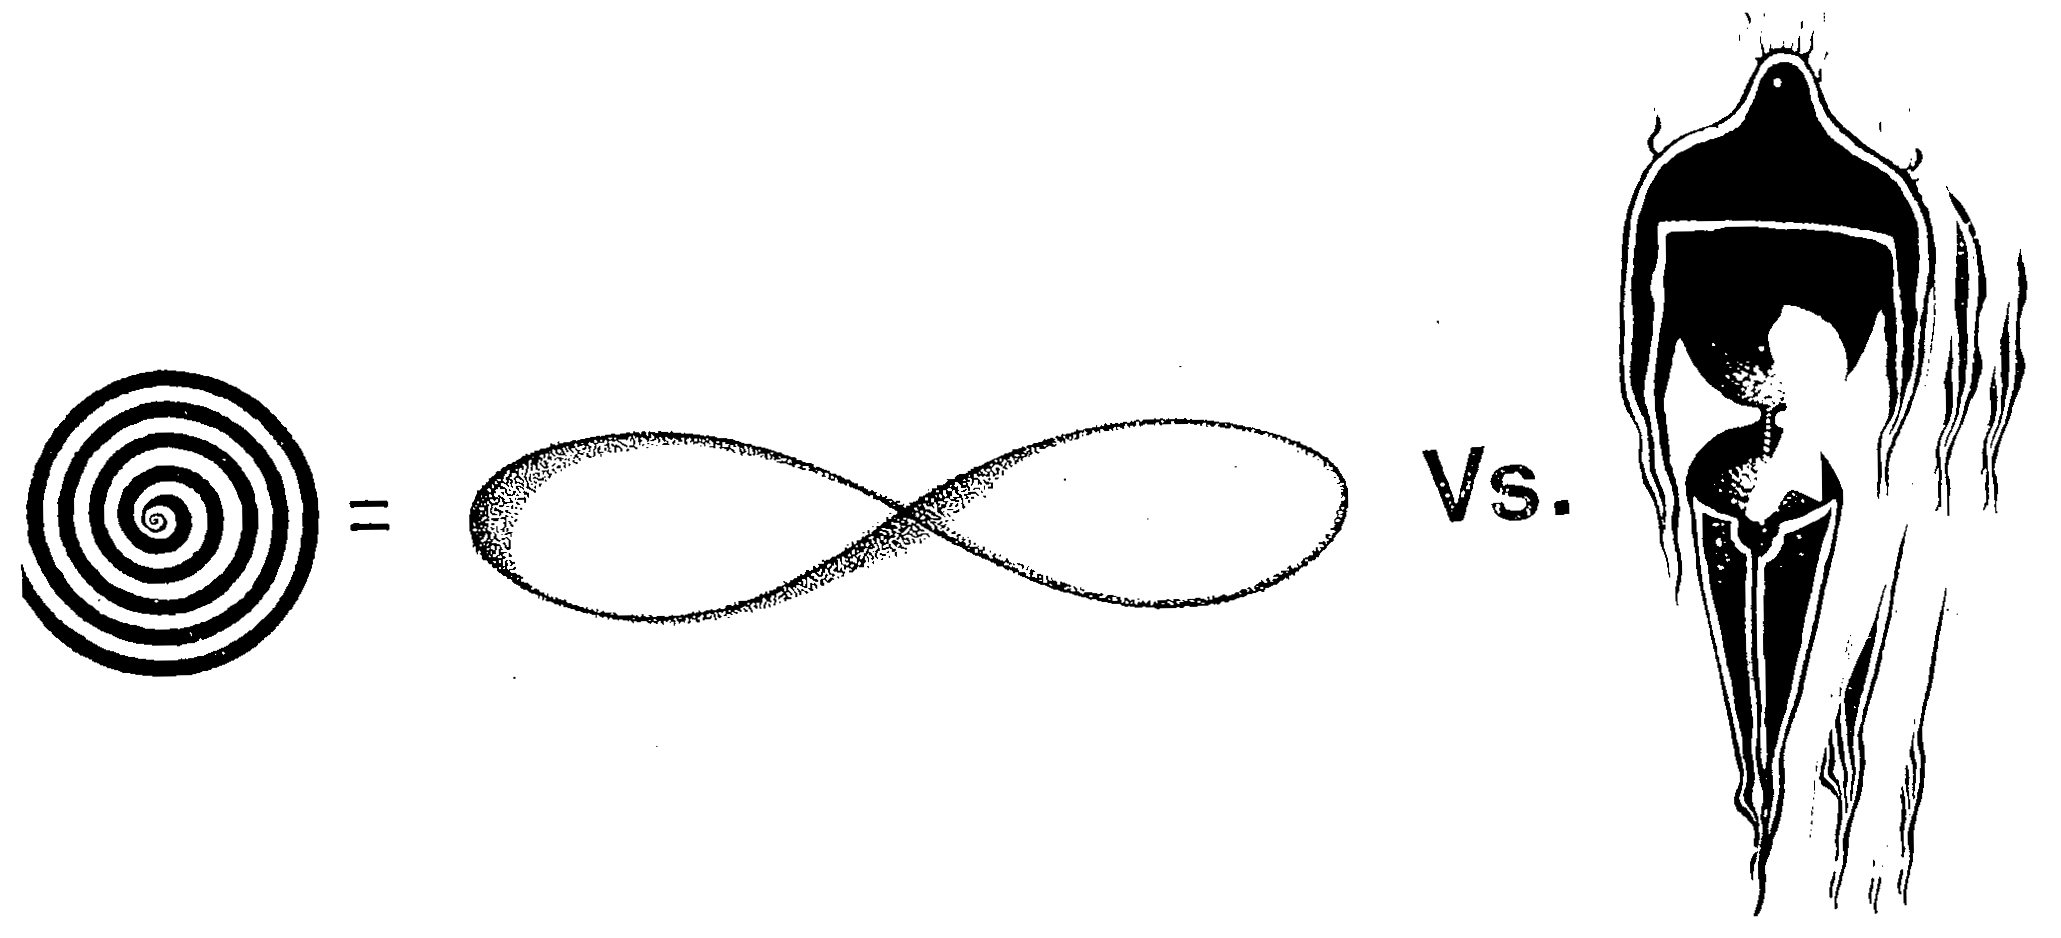
\includegraphics[width=\textwidth]{./images/inf}
\end{center}

From antiquity in the Middle Ages, the metal lead and the planet Saturn sometimes they contradict themselves getting united in a series of correspondences in the middle of celestial and terrestrial spheres. In the middle of what it is not visual and his works in the middle of matter; this complex system of equivalences affinities and allegorical movements, religion, mythology, philosophy, history and believes of diverse civilizations are viewed interrelation in the One: “THE MONAD.”  [According to Dr. Flash Ipondomo, Liebnitz erred! In other words he fucked-up!; the subdivision of matter is infinite, as it is infinite the macro and micro-physical world and he (the Doctor) expressed this idea with an original and elegant graphics (??). Which means that there’s no beginning and no end. Up to this moment, the last scientist Peter Higgs has discovered a tiny sub-atomic particle, that was called “The Particle of God” And Dr. Flash tells us that there is more and more small particles which he would call “The particles of the Devil.”  The “Big Bang” is a joke!! Only the life of the individual human being has a beginning and end!! Speaking in marxist terms, now in a more philosophic terms the human can get into immortality (in certain way) through their deeds, but that immortality has to be preserve by the ones who were left after his or her departure.  

‘In the Middle-ages alquimy, the metal lead and Saturn were central elements in the literal and metaphoric understanding of work (??) It is a fact that Anselmo accepts the functions of lead as the most considerate dense sluggish metal, and on top of that, resistant to change; lead, it is the substance that preserves energy or power, specially as the material used to construct shrines or lockets, coffins, etc. It has associations for conservation but also for destruction, it is a metal of a supreme paradox…

“Lead the most mortiferous metal as toxic as Uranium or Strontium 90: Dangerous Isotope, a product of certain nuclear reaction. Lead has literary meaning, yes!! But physically is another matter; the alquimists wanted to turn it into gold; the most precious metal, symbol of wealth and power, representative, emblematic; The one which is used to buy human freedom, dignity and body. All this is reality-fiction because particularly gold doesn’t have other essential function as an element to sustain life. We coming back to the Golden Calf; the one Moses issued a decree of crime its worship.”

‘Actually its worth is only fiction, manipulated, its physical contact inoffensive, is just romanticism! However lead has a powerful force to cause illness and death knowing that its contamination is lethal, how it is possible that is used to create objects that are supposed to be in human contact knowing how poisonous it is?’

\ornamentbreak

When Egon finished reading this brochure which he found on the floor of the shop, he was surprised and said to himself; “Okey everything is Okey, but at the same time crumbles because visual art is visual art and these paintings of sloppy craftsmanship, don’t have nothing to do with what he had read; all those writings by brainy hack writers, obsessed, paid to write an advocate defense that is useless. The writer becomes a kind of priest as auctioneer, and the “artists” kiss his ass. Art is sustained itself by its qualities that if they are real, they are transferable and imperishable!” He thought, crumpled the flyer and tossed…

\ornamentbreak

The foreman of the shop used to come to check with his expertise eye everything that was produced, and that was how Anselmo’s orders were getting accomplished, Egon was running in the mornings and sometimes he would walk to Wanda’s house and he waited for her, leaning on the new Opel and from there to the atelier. She used to offer him a lift and asked him to wait for her, that by all means she would give him (un aventon de tripas, push the guts), Egon blushed by her much attentions…

‘Few realize about the functions of art. Art how has the opportunity of fulfill many deficiencies and not only satisfy the aesthetic experience, but to call the conscience and be a witness of the futility, cruelty and venality, etc. Art is the mirror of man; art produces reality and frees man. Let’s examine an art work and it could be that we may fall in a rapture by the impact of its beauty or truth.

However the idea of beauty changes over time and this is something that has to be present in our judgment. In the visual experience exists what we call superficial decoration and this is very different from the experience that makes you think, an important element in the aesthetically satisfaction, what we have in front of us is a document that portrays an imaginative artist, complex and interesting or an impostor that tries to impress us and at the end portrays himself as an Alcornoque. (Charlatan)

‘What are the instruments we have to judge an art work? We have the accumulated information that has prevailed; we have sensibility, the awareness of the history of art, psychology, culture and tradition, connoisseurship and science, etc.’

‘We are in the middle of special phenomena in this epoch; the flood gates are open, the Pandora’s Box has been forced open and the confusion of VALUES is present and pervasive in Contemporary Art and in everything. There are many Charlatans and the ones that profit from this confusion are the ones who had created it; galeristas marchands d’art in high-places by a coterie of gloomy accomplices, which are the art-critics, museum directors, advisers for the acquisition of art works, etc. At the end the “artist” allows them being manipulated and produce what his owners ask, all of them are in this business of deceit; who’s responsible? The public that swallows this crap? But  there is no question all of them had given their ass to the Devil’ 

‘The objective is to catch insecure fools with money, this “artists” work day and night, well not they, their slaves and they produce in factories the staff what they call “art”; they have to do it fast because another artists (conartists) manipulators had created an economy like a soufflé of gas to command steep prices for Nothing, that means that we had entered in the dimension of the value of Nothing and we know that nothing is shit! What a contradiction. Today to enter in the art market is dangerous because it is a place with no regulations and the prices could be any prices, all depends in the apparatus of advertising and promotion of smoke.  It is a game of smoke and mirrors, it is the place tailor cutter for the creation of a Myth; the worth of NOTHING!! Sometimes in the art market appear truly art works and legitimate they could demand ANY price, there is not a limit. People that pay high exorbitant prices for trash, well they deserved to go to HELL!! They fucked-up themselves!’ 

\ornamentbreak               -0-

‘It is eight at night I just got here, I walked from the atelier to my hotel, I came thinking about a lot of things, my head started to be engulfed with shit, I don’t know if this is because of the impressions of the last moments today at work, I don’t know if it was because Anselmo’s attitude, he didn’t addressed a word to me and they talked and talked only in German, I was in the middle and all the gang was there, Wanda, Lina, Georgy, Stefan das Pferd and I, it was ten time when Anselmo arrived with Lina, they spend the day in Gottenheim. They arrived when we were taking a brake from a long hard work day; at that time I was ready to leave, I had already changed my clothes I was just leaving when Stefan appeared with the tea, and he suggested honey and rum to warm-up, and I said Ok! Anselmo arrived smoking a huge Macanudo and I thought this guy is Ok now, he got out of that “bitch” cold, I think? Then he make jokes with them, they talked for a long time and he never talked to me, joke after joke with his slaves and he ignored me, then the colloquial idiom I couldn’t understood, I felt like shit. I have been practicing my German with the tapes and everything seems easy but listening these fuckers, pas, pas, pas I was left out of the loop, I noticed that they dragged the words in such a way trying to be apart from me! I thought…

Yes today was a day of a lot of work, yesterday I helped Georgy to make a book, and then I make one alone, I wasn’t very glad. The welding work was ‘rustic’ that was what Georgy said, however, it was a big problem to unroll the big amount of lead, then to cut it after the precise measurements etc. Then to fold every piece by half and make round the part where it is going to be fold, then the welding. I did it myself all, the day went by and I was enthusiastic. 

I left all this crap, Wanda was urging me to go to Heildelberg to arrange my legal situation, however I don’t know from where this feeling of doubt comes, I been thinking about what Wanda said, the day when I was introduced to them, that it is difficult for an artist to work with Anselmo, and it is true. I had been consumed by envy, knowing that I could manage this enterprise (rollo) in another way. There is no doubt that I had come to get a doctors degree with Anselmo.

Today I had to use the goggles to protect my eyes when I was welding, Georgy doesn’t use them and it is a risk, all is Ok but I have to take precautions… I think it is premature to make a judgment about my coworkers and about Anselmo as well… I only know that Anselmo has been very kind, inviting me, and on top he pays my hotel, he makes me partake of his creative process, and I collect information, or he did make a mistake and he was ultra naïve to let me get into his domain, to me, a Tenochca Spy? I’m starting to feel somehow strange his attitude, it is as if he has hesitated and finds himself in a crossroad and he feels that he fucked-up! I am afraid that he is up to decide the APO, again? (The Apotheosis of the Terrible Drama)

‘Today was an incredible day, the warmer sun got in by the main gate and the light invaded all the studio-atelier factory where we work, the paintings acquired a strange resplendence; too dull, and I noticed it it impressed me a lot, they were amorphous stains, the magic had disappeared, it was a strange day, I had to fight the fucking lead, I was uneasy, everything looked like a sticky mess! A nightmare, horror!!’ (Un cauchemar!)

\ornamentbreak

‘I’m trying to organize my ideas; it is 7:30 in the morning. I’ll see how my enthusiasm is for today. Today is Mittwoch definitely I cannot go to run, actually I’m not afraid of the cold but it affects me and I want to avoid it. This Saturday and Sunday past I went to run, I felt I was dominating this fucking ‘sonababiche’ Buchen cold, but after Monday I felt myself affected, I have stuffy nose and mucous in my throat besides I keep wrestling with this bitch lead, ‘sonababiche’ lead, I think that there is a no-way-out, today I’ll try to probe my coworkers my worth, I’ll see what was the Fafner’s opinion. When I’ll be back at my hotel I’ll try study with the tapes…

\ornamentbreak

‘Today I awoke all soared, the fight with the fucking lead is fierce, little by little I have been snatching the secrets of this miraculous metal; it is so docile I had capture the impression of its richness. At this point I can imagine that Anselmo is nearsighted and I don’t know why at this point he doesn’t have an assembly line and machinery like in the Krupp factories, where they fabricated panzers… I’m writing this in the restaurant of the truly giants. Other observation; I had noticed that here and there and at the shop  everywhere everybody smokes like degenerates, simply the ashtray at the shop is a can of about five gallons and is already full of ash, probably this ash is used by Anselmo, no doubt. I’m impatient en el Gulag del arte “Die Bleikunst”.

\ornamentbreak

‘Almost 7:30 at night, Armin brought me to my hotel, I like this kid, Anselmo pushes him hard, he is a young, coarse man, very diligent, willing to render service, he doesn’t talk too much but his personality is likable, he wears “sturmtrupper” boots, rough cotton pants, leather suspenders and a big buffalo jacket, he drives a Fiat all paint flayed-off (despellejado?) with opaque windows I don’t know how he can see, he is a good kid. Today is not cold as this morning but I had to hurry up and get out of Vulcan’s shop early. The day unfolded fast, it was around 8:40 in the morning when I rang at the Palace of Lead, soon after some minutes the gate was rolling miraculously, I am aware that a thousand eyes are watching my movements… When I was walking towards the studio I gathered dry leafs and some diminute beautiful pine cones, cute miniatures in comparison to the huge animals from California, I remembered the one that architect Ms. Maëlstrom brought me as a gift from her trip to Yosemite, she told me she found it at the foot of El Capitan.’

‘I waited some minutes, I had crossed (el pueblo) the town, it was still cold, and it had stopped me to run. Today was another day, another fucking day struggling with the fucking Anselmo’s books. I did the covers, it was hard, the material is docile but the way it weights the ‘sonnababiche’, I dressed up my working clothes, I got into a white smock, Stefan das Ferd told me that I was a doctor and I answered that I was (El Medico de las Locas) the doctor of the insane women”. Stefan speaks Spanish and he is kind, amiable, Wanda told me that he is the guardian of all the enterprise, I think he lives with her, maybe he is the one that is laying her. Yesterday I went to wait for her and he came together with her, of course he deserves her, he is a nice kid. I had observed that Anselmo is kind of dumb. (pendejón) Stefan and I will be friends, he is intelligent the other day we started talking about the Mad Bukowski, I think we can talk more about him. Anselmo came back again smoking a big cigar, and later he was coughing like crazy, probably he is not well, puta!! He doesn’t learn…el pendejo! 

\ornamentbreak

‘During the morning, I finished another book and this time it was easier, however they are very heavy. I was thinking several things… How is it possible that if Anselmo has already an established name in the market place, why he doesn’t produce these books in an operation in line, like the Fords are produced, eh? He?
‘Armin was working with me, I cut and folded, I went organizing them by bundles or groups, I think I was pushing him, he is ahead of me by a nose in matters of bestial physical brute strength, etc. The morning passed fast and I was sweating with the lead, around one, the beautiful Lina called us for lunch, I was starving like Marvin, I was thinking who was going to cook? According to this Wanda wants me to cook but not today, Eh?’ I can just tell her that I had to prepare some stuff and that I had to have a “Brainstorm”, what about some chicken livers with brandy over spaghetti or some Nana tacos?.. Eh?’

‘Stefan das Pferd prepared a wonderful lunch, complex, very German; an onion pie with ham from the Schwarzwald, we accompanied it with some kind of new wine that tasted to me like Tepache but from grapes, I know Tepache is from pineapple and is not sparkly like this one. Lina prepared a grüne salat, I was impressed by it looks, (which, the salat or Lina?) we had lunch again at the conference room. The stupid Karl almost throws-up, he eats and smokes at the same time, everybody smokes; Anselmo his habanos, Georgy, Marlboros, Lina some small black cigars. After lunch we went to work; Anselmo told me personally to make the book number sixty, Armin and I cutted what goes in the middle of the books and followed-up the progression. Karl and Anselmo were checking some paintings and were assembling them, well Anselmo was only giving orders, I didn’t see him touching anything, then he disappeared… The time was passing very slowly until the tea time. Wanda called us, Armin played dummy and kept working, he doesn’t like to socialize I think he feels himself different, he is “rustic”. Something strange happened; almost all week nobody talked to me, they talked among themselves, and nobody said a word about it, I felt isolated by these fuckers.

When we were at tea time somebody called from New York and Wanda was saying to that person that this art piece was already sold, and that the other one also and bla, bla, bla, the clients will pay for the freight and the crates etc, etc, and this and that, big business, I looked like a Chinese, full of envy, I know Wanda was right; it is very difficult for an artist to work with Anselmo and realized that he is a wizard to make money, with shit!

I have been studying this operation, for Anselm it is very important to know everything that is written about him and his work, and he systematically collects it, and what is published as well, he gets magazines from all over the world, and he is aware shrewd, maybe he is afraid to be unmasked? He knows very well that he has to do it now!! And saturate the market, but something in his mind worries him, what? Posterity? To be investigated thoroughly? And being turn only into a footnote? Oblivion? Ridicule? Ass-hole? A clever idiot? Like other idiots Koons, Warhol, etc...

\ornamentbreak

‘Today at tea time I was leafing through a magazine that Georgy brought from the mail box; “Volkstelles Kultur”, it is a very expensive magazine but I liked a lot; there I saw another guys that are working with lead, that means that we are in the epoch of the “lead”, it was a bilingual magazine, then we got back to work, I’m worried about my health knowing that lead is poisonous, its toxicity is dangerous; you touch it often and you get cancer, no matter how heavy it is, its all over everywhere in the studio, the miasma of lead floats… How?’

‘The huge studio is divided in four principal parts, you push open the gate and you cross the patio at the entrance, at that moment you start working for Anselmo; printing with your weight all the lead that is scattered everywhere. The visitors and autos etch the lead and then when is ripe, the slaves pick up the plates already processed and then put in place fresh ones. I think Anselmo is right, there are so many that would like to steal the blue prints of his creative cuisine, and the formula to convert lead or trash into Gold!’

\ornamentbreak

‘The office is Wanda’s kingdom; from there she watches all the property trough her monitors; the cameras look all the space; the conferences hall, the first huge shop, the second with the water pool of black and rusting metal scrap in it, then the huge easels, bench and work tables, materials, a thousand things, then the private Anselmo’s rooms. Wanda told me that there he writes and sometimes he spends the night there (what in the fuck he writes about?) he reads as well. It is his spiritual seclusion. (?) I couldn’t penetrate there but I imagine he must have his library, his computer, and the monitors that watch all the operation, probably he has Persian carpets over a polished beautiful, rock floors, his sculpture collection and probably Durer’s paintings (his Nemesis). I think he doesn’t like Picasso, one day I heard him saying awful things about the malageño. Probably he has works by the great German painters: Holbein, Caspar David Friedrich, Altdorfer, Baldurg, Cranach the Elder, Master of the upper-rhine, etc, figurines from Oceania and Africa, maybe ivories and china, jade, etc.

The big doors that can be lifted and can allow the big trucks get into the edifice, so they can be loaded to carry the heavy and enormous metal frames, books and shelves to be sender away. The garden at the back of the building, there are sculptures in embryo that are corroded by the elements. In the third studio more paintings in progress, electrical saws, working benches, the welding department where the metal easels are fabricated, the exposition tables also made of metal to support the weight of this infamous and diabolic plombastic (?) vision!!

Fricko Kiefer, has turned himself enigmatic, mysterious, what he wants from me? I told him in my letter who was I, suddenly I feel some coldness in his behavior. (Le apesta el culo).

\ornamentbreak

“Black putrid flowers” was the idea that came to my mind this morning, I have been thinking in the observations that I had done in the studio atelier, I read in a catalog what this water-pool of black waters signifies for Kiefer; is the source, in the middle of the second studio, (the source of a plethora of ideas from the fertile imagination…) I thought it was an interesting idea. What I have confirmed is what I did 15 or 20 years ago, why did I stop exploring these possibilities? I wasn’t prepared? Mi vision was foggy? What distracted me? It has to be proof by the burned drawings, then the metal works with the application of different materials, the punched copper plates, etc, the montage of different elements looking for the image and meaning. The experiments at the Santos Balmori’ advanced shop, etc.”

\ornamentbreak

‘Yesterday we worked like hell, we gave ourselves punishment, Armin tries to show off at work, Georg works also, yesterday I noticed he was not in good humor, like saying “look at me but don’t touch me!” I didn’t say anything until night time, he said that he was bored and concerned, he wants to go to see Ursula his girlfriend and I don’t blame him I would like to see Maine in San Francisco. We completed 6 more books but we need to finish a lot more. Today Georgy would not be at the studio, Karl would be the foreman and I will endure, but I will do my best, I think that I had gained more than what I have losted. I’m still sunk with ideas, his indecision, my indecision, what’s going on?

‘Here in Buchen I’m thinking about San Francisco, my mind flies to my studio at that cul-de-sac at Pajaro 5, my hideaway, my domain, I’m thinking about things, how they were happening, I remember J. Reed when he visited me, I was telling him, that I could still stay in that ivory tower for another 20 years observing the human fauna, and there among my art collections, books and my work in progress… Suddenly, now I am behind the overhead scenery of the art in Europe.”

\ornamentbreak

‘Days have been passing sometimes monotonous, other times exciting and interesting. Kiefer goes out of the country, the big trucks come and carry away the works of the noted master and we won’t see them again. It is 7:05 I just arrived to the Giants Hotel, I walked from the atelier it was not cold at all, a thousand ideas are boiling inside my tête de Mouche. Suddenly Anselmo comes up with the ideas of telling me that I am not the person that he needs in his shop and he cannot employ me… Possibly I was waiting for this and I was thinking to abandon the job but he came first, and of course this decision has to do with something else, everything up to this moment has developed smoothly. I want to know what was the real motive of the change of his mind? These last weeks I had worked my ass off to accomplish the job, however his decision is final! Well he has asked me to come in the morning to get my pay. Anselmo is a shit-head bastard!! Everything is illogic and absurd I don’t understand what in the fuck did him make this change? I already had plans to stay and appropriate all the operation, there is no doubt he leaves me (descojonado) with no balls, however I have to capitalize this breakthrough!’

\ornamentbreak

‘I am here at my hotel feeling myself like shit, this fucker had the capacity to change the course of my plans.’

\ornamentbreak

‘It is 4:15 in the afternoon at last I’m escaping from this rotten place of mythologies, I have in my mind very present the images of Kiefer’s art, there is no question of their power of fascination, maybe the fact that they are so phisically big(?) 

After the decision he had, I have no other alternative than to get out from the castle of Lead. However I want to know what was really what make him to take this decision? Out-of-the-blue while I was finishing another book he came to me and told me that he doesn’t need artists in his organization but slaves who he can manipulate, that he doesn’t like to hear commentaries regarding what his factory produces and not even opinions, he said 'the slaves have to be automaton, and he wants to know what I write about so often? I was astounded, at that point I couldn’t answer, finally I said Ok. Some days past I had already felt certain insecurity, something sometimes my stay there was shaking. Then he asked me to stay more days and I said no! His decision was final and mine as well. I crossed the huge studio, I passed by the lead heaps, I saw for the last time the big paintings and went to change my clothes, the day had been hard I did 2 pairs of book covers and I was satisfied I was thinking hard about all the possibilities, I didn’t take photographs but I have in my mind the details and the blueprints. Stefan das Ferd was coming down the stairway and asked me if I had worked? I told him yes and I was leaving, then he kept asking me and I told him more or less what the situation was, he said he didn’t understand, he said “the German mind is full of shit!!” I told him that in this moment Kiefer is the Ogre of the Castle of Lead, and he answered “Richtig!!"

‘I dressed up, I sighted and entered into the office, Yenti (?) was there, Karl and Kiefer, Wanda was playing dummy, leafing through a note book (also made of lead) I went out behind my dark glasses and I said “until tomorrow” and everybody stupidly in chorus said “Bis Morgen!!”

\ornamentbreak

“Reflections… At Finkelbach;”

‘I’m trying to reflect, soon I will be going to Paris to see Paul. Ok I’m here sound and secure, it is 7:30 in the morning, it is a glorious Saturday. I was awake at 5 and turned on the night lamp, I went through the Stern magazine, The Star, they talk about Scorsesse and his film “The last Temptation of El Bato Christ” besides that, some photos of some broads that fulfilled my eye, then I started to leaf through the Beuys book, I had decided to get up and do my exercises, Holmer and Elke and Bruno went out early they will return later, we will have dinner together, I had invited them to a restaurant here in Finkelbach, I will go to Paris I had talked to Paul and he would wait for me at the Gare-du-Nord this coming Monday.’

\ornamentbreak

‘I’m trying to rethink and analyze all these situations that had been developed, I think about Kiefer and I know that I have to be patient with him, of course the motive of this decision was not what he said to me but another completely different I’m sure, he realized too late that a Tenochca spy had penetrated his mythological organization, a spy inside the world he has created, then I thought when he asked me if I had a photography certificate, at that point I knew that he answered my letter under the influence of a mistaken idea. He uses two students of photography and he manipulates them any way he wants, he told me that I could not get into the photography department because he goes there and orders how “things” will be done, “effects” in this case, but what was the problem? I didn’t have any critical authority for his “creative” caprices and opium trips, whims, or fancy, then he turned paranoid ? But why? He was the “boss”. I realize when these kids that study at Stuttgart, they were impressed with my questions, judgments, and opinions, that was the “smoking gun”. Then when I examined and analyzed the big photos out of focus with the horrible opened grain, the stains, not well fixed, half-ass overexposed, solarized by mistake (?) As one would say “he was another ass who played the flute” like Warhol? I thought that all was well thought out, calculated, studied, directed, etc, and now it happens that it was Anselmo’s secret formula, Ja, Ja, Ja, of course he felt himself vulnerable. But why? This is infantile, he could utilize me and utilize all this years where I had experimented with many options, the same thing happened when I saw Richter’s work it was déjà-vu. And this shitty art critics, they don’t know nothing and are impressed by Kiefer or Richter only because they are Germans, because Germany has produced Mercedes-Benz and Porsche, or MBW’s and Audis, ha! But it has also produced Beethovens, Luthers, and the divine Dürer, Gutenbergs, and this is not a reason to accept a half-ass mediocre; even if he is a German!!

‘That Dürer is a hell of a painter, marvelous draftsman, sublime engraver and K. and R. are just a mockery of what art is, and they know it. Why they had surprised the fools? Because the public is illiterate? Stupid? Moron? And the circuits of museums, art critics, galerists, art marchands, have done a great business of the ignorance and they don’t know anything, they had bastardized the sensibility and this is very sad; those horrible abstracts made with squeegees that Richter sign.

\ornamentbreak

EXTRA!!    EXTRA!!!!  EXTRA!!!!   

Embarrassing and sad the presentation old old Richter !! He allowed a crew to film the execution of his formula to paint . He was armed with a huge squeegee producing paintings ….Another Charlatan. His impotence was notable …..He was lost ….Wandering in a strange world of smoke and mirrors …With a gigantic squeegee, pathetyically where to floppe it?\\
\\(Painting is the Divine Art) Rinaldo della Robbia .Art Critic.
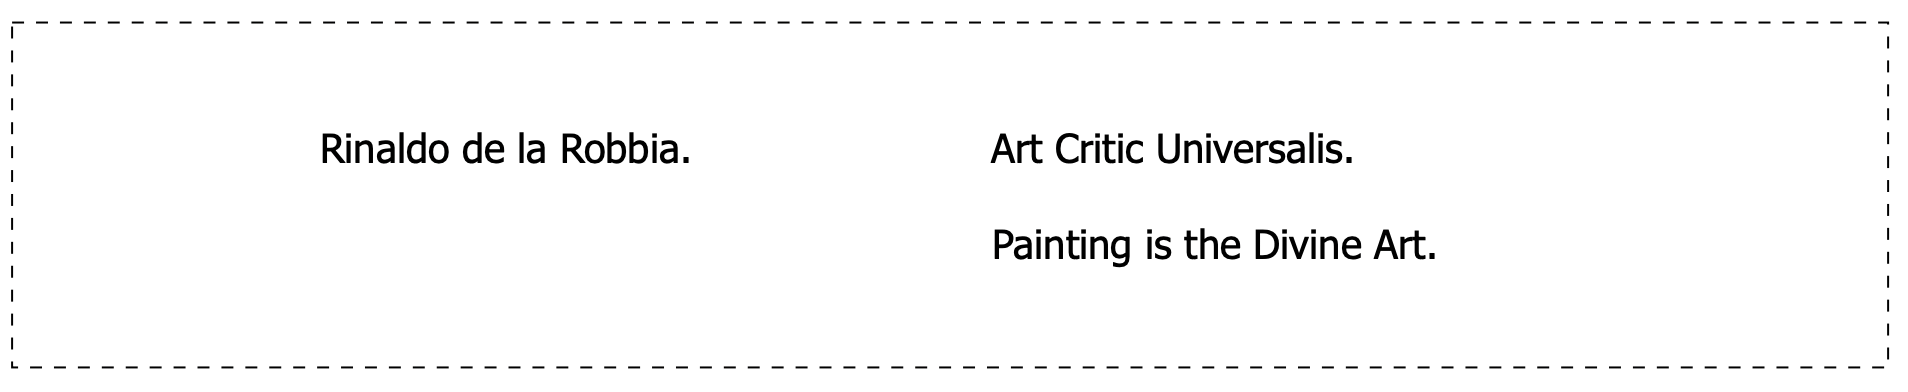
\includegraphics[width=\textwidth]{./extra}

\ornamentbreak

And Kiefer’s horrendous caricatures of the notables of Germany, together with those horrible “watercolor” or “gouaches” he calls, namely half-ass photos smirred with mud, fat grease, hair and shit and straw, there is no doubt that we live in the times of the Charlatans and fake painters.” 

‘After all this the kids talked to Kiefer and he had a fit! On top of that all that time, hours in the archives; Wanda probably told him of my attitude. I went to the bottom of heaps of documents and photographs, digging and revolving his guts; his mythology in the bud, going to the meanders of the molecular structure to check if there was magic or no: Maybe magic is a product of advertising? Obviously! In my collection I have close to me my beloved Dürers, Posadas, Hogarts, etc. And this makes me noticed the difference between the real ART and the mediocrity of these fucker phonies!’

\ornamentbreak

“I arrived to my hotel and I realized that my mission in Buchen was finished, then I called Holmer and kindly told me that he will come for me the next day, he asked me to be ready. I turned on my sound system and started listening to Yepes and Paco de Lucia… I started to suck brandy and little by little I was sinking myself in that kind of subliminal feeling that Buñuel talks about, I kept thinking how three months had passed in that A. Kiefer’s Castle of Madness…With the ash up to my balls..."

Next morning I got-up little bit later I was awake at 4 and I got up to write, read and then I went back to bed, so I got-up at 7. To the dining room I arrive at 8 and had the same breakfast I wrote again and followed up step by step a plan, I went to the stationary I bought post cards. The morning was beautiful… I saw the things very clear and I couldn’t believe, I imagine Kiefer with no balls, a pathetic case I kept thinking. Then I went to the bank and cash Anselmo’s checks, then the idea came to me and I went to gather dry leaves which I would use for a Buchen painting. 

\ornamentbreak

‘After I bought the post-cards I crossed Marktplatz and went to the post and wrote them there, I was dressed with sobriety. The clerk at the post was kind, I paid and he told me he will put the stamps on the postcards I said to him “Danke!” and went out, I was carrying my camera, I had the idea of taking a photo, the weather was nice, the summer was around the corner and I walked towards the Castle of Lead… I observed the small villa, I look hard in all directions, I wanted to record the image.’

When I arrived at the atelier I pushed the button, I was looking for the last time Anselmo’s building. I noticed in the middle of the patio a new Citröen, the biggest with Netherlands plates, then later I knew that Anselmo was attending personally in his studio. They were collectors of Kieferian art, they came directly to choose from the new harvest from last week, Kla! Wanda welcomed me very kindly and told me that she was sad and that she talked about it with Stefan das Pferde,  she said that she was sorry and asked me that I should talk to Anselmo and ask him for another opportunity, “What?” I told her “it is not possible!”, well, we talked and I realized she was really in  commotion, her beautiful eyes were red at the point to cry (?) I thought she was going to fall on her knees and ask me not to leave her!”

\ornamentbreak

‘Suddenly a fucking cold attacked me out-of-the-blue, the shitty germs came to me and snatched me. I got this cold about a week ago in Buchen and I couldn’t leave immediately to Paris, but I’ll do it soon, I’m listening to Yepes, in these days here at Finkelbach I been painting the picture I promised Holmer as a token of my gratitude to his kindness, I’ll finish it and he will take me to Mannheim where I will take the train to France.’ 

\ornamentbreak

‘The day that Kiefer came back to the shop, we knew it right away, the aroma of his Cuban cigar arrived first. We felt immediately the presence of the German master when we breathed the essence of one of the cigars from Pinar del Rio, these cigars are unmistakable and were sended by the guerrilla leader, Anselmo’s personal friend. Anselmo came strolling by the middle of the shop, he looked everything and said “Ausgezerchnet” and immediately disappeared, it seemed he had an important appointment, he asked Georg to take over the production. And the Georgy that seemed so inoffensive and sweet, started to walk from one side to the other, exclaiming “arbeit!” “arbeit!” “arbeit macht frei!” And we heard his boots stomping the floor, the sound was frightening… It was 12 at midnight and we should finish ten more horrendous books, and we were signing in chorus! With saddened voices… A capella…”

“We are the midget-slaves 

The ones which work at Vulcan’s forge, are we Kieferian slaves?

Yes, we are! Kieferean slaves!!

We  are forced to work our asses off

Kieferian slaves… slaves… slaves…

For Kiefer and the fucking Lucifer…”"Ojete!!" (ass-hole)

\ornamentbreak

In those days it was tension in the air, Lina seemed reserved and Egon was observing her, distorted, the lines over her face were profound, more visible, her eyes with shadows, what was happening? Her glassy glance, it looked as if she had been in hell like Rimbaud. 
                              -0-
                              
Then certain frictions came into play: Egon had an altercation with one of Kiefer’s assistants; the photographer; Egon criticizes one of Anselmo’s works. 

Egon told Helmut that Kiefer doesn’t know how to draw, that it seems he has apoplexy, Helmut said that, that is not important because the maestro sells a “watercolor” regardless made half ass, in 20,000 DM and a photograph for 13,000 DM and that it is important (?) Well just think about those aberrations called “watercolors” and don’t mention about the messes he does to photographs printed half-ass. That’s too much! And of course Egon thought that he was cornered by the shrewd Helmut. Then gave course to his ideas and said that he admires Kiefer because he knows how to manipulate his success and that he [K] got to the moment where grandieloquence and bull-shit impresses and that is a leaning point, but is only bluff, he has builded a soufflé and the leaning point works as a Fulcrum!

Beuys has all the merit and Kiefer has used it in his own benefice, he has capitalized Joseph’s teachings, then his opportunist thing with the Jewish affair using his pliable nature… Egon asked Helmut and insisted that all of this discussion was only between them, nevertheless it got to Anselmo’s ears. After this incident the plan that Egon had, started to change. First and foremost, when he knew that he could penetrate into the life of one of the most famous artist of Germany’s postwar era; Anselmo Kiefer. Everything started to crumble; his infinite plan was remaining unconcluded!! Egon knew he could manipulated him for his own benefice, utilize him, it was in his own right, but he was betrayed by his emotions, he should have stayed quiet, no words… He erred, he arrived to the studio-factory, he was working diligently; then in several occasions he wanted to be ahead showing Fafner that he, Egon, could be one day the chief in charge; By his own initiative he moved or fixed something that he thought was out of order; and that was anathema, the damned cameras started to take note… they started watching him, they were at least 8 cameras, at the beginning when Egon saw them he didn’t care, then later he verified that the fucking cameras were reproaching him…(?)Fallowen him, stucked on him like glue...

In the third studio-gallery there were 4; this was a huge oblong place cluttered with some finished works and other in progress, many of these paintings were bizarre and absurd with ideas that I think had no aesthetic value. Simply huge and also huge photographs and toys as well enormous; as if they were conceived by an idiot kid non mentis compass (?), grotesque!! As the abortion of an imbecile and troglodyte mind, something INCROYABLE!!; Like one abomination that pretended to be an automobile made of pieces of garbage, but maybe because, it was an aberration, was a touch of genius? All this conception ended with these aircraft models of jet planes as emblematic and symbolic metaphors of what? Half-ass pipes of stinky sawer filled with long hair that was hanging by the jets (?) then the paintings with ash, lots and the ones covered with straw, lots, of course!! STRAW!! PAJA!!

Anselmo started to be suspicious about the Mexican craftsman, thinking that possibly Egon was a Tenochca spy? Then for sure the eyes of the security system surprised him touching and analyzing at close range the paintings, there were some specially with gold ingrained in its molecular-fisical structure; gold like “carrot”, Kla! And lead, acids corroding the matter and then again straw, in abundance emblematic! Kla! Metaphorical! Analogous!

Egon knew somehow that Kiefer’s alter-ego was Dürer but Egon believes that instead to be his alter-ego was in fact his Némesis. Dürer is a super painter! This one is an ALCORNOQUE (?)

In February the crisis started, Kiefer told Egon back in November that he would be on trial for one year and if everything was Ok he would be in charge of the factory, Walter decided to become an artist as well as Kiefer and he will be gone.

In those last days Egon was surprised when he saw Kiefer was coming out of another bitch cold, showing off a big (macuche) cigar; it was one from Pinar del Rio or a Macanudo, but how was this possible? Just some time ago he found him with ghastly running nose! He was blowing his nose, his eyes were red and coughing, he was a mess. Egon told him that he was carrying some homeopathic medicine called “Echenocia” and he offered it to him, he accepted and went home to get some seating’s baths, etc. “Poor guy!” Egon murmured… Anselmo was looking very bad!! 

\ornamentbreak

This performance was happening in the first gallery, it was about 11 in the morning, Kiefer ordered Georgi to bring the lift, and the apparatus got in like if it was activated by efficient robot.

Kiefer got on to the special platform and ordered to be lifted to the heights, quick!!! Schnell!!!

The enormous steel curtains that separates the other gallery where the lead books have been fabricated was entirely open and everybody could see what was happening… ‘we heard the mechanism of the lift and Kiefer was going up to the heights, meanwhile other assistants were extending on the floor a huge canvas with ensembles; wood and more lead, this piece was in progress and was being adjusted by the German master.’

Egon saw everything; now Anselmo was going up like in the legendary messianic Ascension and it seemed that even little clouds and a sunrise was part of this image of anthological míse-en-scene status: Anselmo magnifically clothed in his zebra robe, projecting sovereign power.

The cigar, and the smoke were making spirals, and the red of the tip like a twinkle light… The German master lifted the right hand and like a beatific gest he pointed to the right… Georgy servile but efficient moved the enormous ensemble piece and Anselmo (expletive) said: “rechts!!” “ein bißchen mehr”, “bitte!” “gut!” Georgi quick moved with difficulty the big piece of canvas trying to satisfied the boss. “Nein, dumb Kopf!!” “Nein!!” “Jetz, gerande aus, bitte!!” “da, da,!” Georgy mobilized himself and Anselmo said “Richtig, Okey!” “Genau, Ok, Ok!” “aus!!” “A la Goma!! Ya!!” (?) (to hell).

Then he ordered to be lifted more and more, until he touched the ceiling, now he was away and tiny, the live little red coal was at the most an incarnate pin-head. The tremendous macuche from Pinar del Rio was still giving smoke signals and suddenly Anselmo started to cough like a madman, damned, desperate!!! Probably he took a long drag from the habano and with his cold, the bronchitis and on top of that his delicate artist inners, this triggered a hellish attack of coughing. Egon couldn’t believe it, how could be Anselmo so stupid, this guy with that big stogie, showing off how important, how “cool” it is to pose in this circumstance; it was like a ritual, coño! ABSURD!!

Now he was red like (el camarón de la isla) the shrimp from the island, and the cough was diminishing him and kept punishing him, he tripped, stumbled, he lost control and Egon from his observatory said, “this fool will kill himself!” the cigar dropped from his hands and Kiefer grabbed the hand rail from the lift, it was like a handle. When the cigar crashed on the floor the sparkles flew everywhere. 

Egon was frozen, in suspense, and just because of this he let the big lead roll get loose, the fucking alloy-lead roll did a strenuous noise, and he did all possible to get it and got it back, then he rolled again. Probably Kiefer didn’t like all this raucous, then he was seen coming down grabbing the lift with his 20 nails, his face was discomposed and the eyes tearful and red, he was angry and was slobbering, fuming!!

At this point other things of no importance but in this context were making weight, the workers after the hard labor sometimes took a shower there, the facilities offered were modern with a very clean white bath room, with lockers and functional benches. Sometimes Wanda turned on the sound system from this artistic complex, and classic music always was heard, from radio stations of cities like Berlin, Mannheim, Bonn, Colonne, Bavaria, etc.

One of the images that Egon was intrigued by, was when he saw in one of the lockers, the one which had one of the doors open and on the metal sheet; some s/m photographs; perverse, of sexual flagellations and domination, etc… But interesting…And disturbing...

In one of them, the biggest; a beautiful woman was tied up and gagged, bent over showing her ass like waiting to receive a good fuck or a good anilingus. The beautiful white gluteus in contrast with black shredded stockings, the voluptuous excellent forms. The zipp-up fastened cords tying the wrists and legs. Egon was in shock!! It seemed he knew that face or it was only a supposition? Those exaggerated open eyes,  looked scared or impatient for the penetration? And a rubber ball in her mouth to avoid the scream of pleasure or pain.

He was there for several minutes fascinated, gone. When Walter at that moment arrives and noticed the spell and asks Egon if he likes it? “Befall dir Sie?” Egon answered “Ja, Naturlich!” Walter.- “Sie ist sehr schöne, nicht, war?”

Egon.- “Ja, du hast recht!” Egon was rapt slobbering, longing…

Egon looked hard; she had bruises, black, violet, the black stockings were in shreds, ripped off… Suddenly the sound of an organ was heard in The Anselmo’s Kiefer cathedral, it was the Bach’s fugue in G, Egon thought about Nemo and said “it was Lina, I’m sure!!”

It had passed already 3 months, Egon did made a resume of what he did and how he worked, of how his investigation was progressing… Running in the mornings, the boredom of the weekends, or to go to a kino early on Sundays, sometimes to go and have a beer in some “Bierstübe”, then going back to his hotel, read, call Holmer, etc. In two occasions Holmer and Elke and Bruno came to see Egon then had lunch and spent good-time with Egon. Then the Wolfes left… Egon kept writing, sometimes he used to call Amerika but he had to take in account about the hour; it is 9 hours ahead in Germany, sometimes he made a mistake. That morning he awoke sweating and then started laughing recklessly “Ja, ja, ja”, “Ja, Ja, Ja” “The fucker is so stupid… Ja, Ja, Ja” It was the first of April, “The Day of the Fool” It was Monday and Egon showed up like every day, Kiefer called him and said.- “Herr Berg!” Then immediately Egon answered “Herr Berga, je vous prie !!”

“Was?” Kiefer answered “was ist das?” “Ich spräche kein französisch herr Berg.”

And Egon continued…

“Yes Anselmo…” Egon answered but he noticed that Anselmo was using the formal in the German language and he felt his heart jumped. Yes, his conscience was betraying him, he knew he was there as a spy and by intuition new that something was wrong since he decided to contact the German painter, he couldn’t understand how all this images that he saw in art magazine and then all these “works” commanded too much attention, something was wrong!!, he confirmed when he saw it at the art show in Los Angeles.

“Why?” And he wanted to discovered. A big conspiration was manifested. And now Kiefer was suspecting that his programmed, his design, was going to crumble and decided to cut Egon off, but it was too late, Egon had already all the information to unmask the fraud of the century. “The Myth of the Art” Anselmo’s!! Of course!!

One of the mottos of our time is to manipulate a double-standard, to be and not to be and Egon was happy because he had discovered that what is believed Kiefer was, is not!! And Egon was ahead of Kiefer because he is what he has always BEING!! Kiefer said “Mr. Monte you are not, what you said you was!” And Egon answered “That’s right, I am not what I said I was, because ‘Ego sum qui sum’ (Exodus III 14).

\ornamentbreak

More and more Egon had realizing that very few people know what art is and in this case: Painting, not even the art-critics and less the art traffickers galeristas and marchands d’art know, the truly art critics are the painters, only they are the ones that can analyze structurally, aesthetically or philosophically the art work.  The good critics render information, data. Probably there have existed few Ortega y Gaset Greenberg Benjamin and Hugues Henrickson.

The official critics only because they had escalated echelons in the museum circuits and had gobbled theories and pseudo-theories and they, the majority doesn’t know what’s happening in a painting. One day he listened to a critic saying that he was not interested in painting; getting himself in the problematic of a painting, that that was too much work, that he was contented only in manipulating ideas from his desk and be on time to a dead-line for publication, and many times he didn’t care what he was writing, sometimes what the product was, was an aberration! And fortunately or unfortunately language is so flexible! That, you can fill-up pages and pages and say nothing, besides people doesn’t read, they are only moved by fashion or by the influences of celebrities. Also the ones who manipulate the culture, and sometimes they get it, they plot with institutions, galleries, critics, etc; They give an ideological or political orientation to art, we can see this in the world of art of today, everybody follows the kids from the New York school. And who’s the cheerleader for this bunch of charlatans? Newspapers, art magazines, etc. They make big names, they blow them up and later they wear them until they fall in oblivion, the works are storage and if are bad only reaches the status of a foot-note, and if are good somebody rescues them and become the discovery of the century; that happened to Caravaggio or Van Gogh among others! Kiefer’s case is bloated out of proportion and his success is understood regardless of the fact that sometimes is confused, erratic, his intentions sometimes surrealists, o dá-dá, impressionists, reductivistas in some cases. And his obsession to obliterate with the grandiloquence that surprises, now if we examine his draftsmanship, he has apoplexy! His erratic compositions, dark, illegible in its facture, he follows Pollock astray, then the use of architectonic illustrations using Speer or taking as a resource the emphasis in the illusion of amplifying the image of the omnipresence, Bombastic!! Something as Monet did, removing the past from Spanish painting. However one of his good hits; his nationalistic ideas when he tried to portrait with those caricatures of the Germany’s notables and adding all that in a mix with Egyptian, Jewish, Mesopotamia and Martian!

Opportunistic? Reverse psychology? The Golden Calf? “Deutschland über alles? All that and more!

Egon was following the dots and spend the rest of the day, thinking and making notes… Then he called California in the United States, his conversation was brief with Madam Gabrielle Brückner, she was sad and Egon asked her not to be worried, he asked also if there was something now… An earthquake , a fire?? 

\begin{center}
    Finally
\end{center}

They said good-bye in a friendly way, Kiefer Anselmo gave several books as a gift to Egon and he said that soon they would see each other again. It was the first of April “The day of the Fool”. From the Giant’s Hotel Egon called Holmer and he showed up the next morning to pick him up and from there, he took him to Mannheim. Egon would take his train to Paris, he had already talked to Paul Nero, the eminent writer and sociologist, veteran of the second world war, professor and lecturer at The Sorbonne University of Paris. 

There were some years ago when Egon was a guest in his house and knew about the great project in which Dr. Nero was working for 40 years; a book that will encompass all disciplines of known knowledge, a sociological structural study of Confucio’s “Book of Changes” the “I Ching”. Elke Bruno and Holmer said good-bye to Egon at the train station, he will arrive in Paris the next morning, and of course in Paris another great adventure… Probably Anselmo totally forgot Egon, but Egon remembers him, affectionately…

\begin{center}
    ADDENDUM
\end{center}

The con-artists and their acolytes profit …Cynically…They produce fast because they had created an economy like a soufflé of gas to command steep prices for NOTHING !! This means that we  had entered into a Dimension of  the nothingness !! Or of air, smoke or ultimately a fart of a beautiful woman in a bottle.

Like flies, buzzing, hovering on top of a putrid rotten pile of flesh creating this conspiracy, consumed  by abject greed, enjoying in secret their accomplishments.

The galleries, merchants d’art  and a coterie of gloomy characters which are: "art critics", "museum directors", advisers for acquisition of art works celebrate  openly  their deeds, the conspiracy is all BUSINESS. The substance of the art object is not important, its value sometimes fictitious it’s manipulated, that is the bottom line.

Entering into the art market is dangerous because is a place where there is no regulation and the prices could be any prices, it all depends of the apparatus of advertising and promotion, scandal and draconian means to capture the interest of the public.

And where are the roots of this chaos? 

The spikes of flash points are with no doubt: Malevich, the inventor of “black painting”, Duchamp the originator of the “ready made”  and Beuys who said that any body could be an "artist!" And the clever idiots to the attack!! 

These three characters created a deluge which has been produced by the imitators which is what is suffocating us!! So many eyes sores!! So much garbage!!

Warhol is a different thing , in the first place he is a product of an accident , he never had a vision , by a fluke he became Warhol. Regardless of the fact that his work is pivotal by the confirmation of the  “pop-market” as object d’art…… Of course there is also an incredible amount of good art out there , and that belongs to the connoisseurs or the persons who are informed and educated and on top ,  sensitive!!

The good art can command any price and the winer would be the lucky one who acquires it, and the crap sooner or later would be abandoned in basements or attics  and will became a footnote irreversible, unless if it is real art somebody discovers it and become the find of the century. Good art is everywhere just open your eyes and be critical! NOTHING IF NOT CRITICAL!! WS.

\vfill

\begin{center}
    A NOVEL BY EUGENIO de ARNAL DEDICATED TO HIMSELF
\end{center}
%%%%%%\lipsum[1-20]
%%%%%%\chapter{Chapter Two}
%%%%%%\lipsum[21-40]
%%%%%%\chapter{Chapter Three}
%%%%%%\lipsum[41-60]
%%%%%%\chapter{Chapter Four}
%%%%%%\lipsum[61-80]
%%%%%%\chapter{Chapter Five}
%%%%%%\lipsum[81-100]
%%%%%%\chapter{Chapter Six}
%%%%%%\lipsum[101-120]
%%%%%%\chapter{Lalala}
% begin back matter

\end{document}
% END THE DOCUMENT